\section{Introduction}
\label{intro}
Social Anxiety is characterized by an intense fear and avoidance of socially evaluative situations~\cite{APA2013}.  Socially anxious individuals tend to exhibit behaviors that are consistent with their subjective states, such as trembling, sweating, and fidgeting during social interactions perceived as threatening~\cite{stein2008,wenzel2005}. Importantly, these behaviors are part of a feedback loop whereby socially anxious individuals experience or imagine rejection from others due to their (perceived or real) impaired social functioning, which in turn reinforces their fears and negative beliefs about the threatening nature of social interactions~\cite{chambless2002,wenzel2005}.  It is therefore critical to detect objective behavioral markers indicating heightened anxiety which may inform potential opportunities for prevention and intervention.   

Traditionally, psychological research on factors linked to social anxiety has relied on laboratory-based methods, thereby limiting the ecological validity of findings.   Advances in recent decades have made it possible to monitor how behavioral systems unfold in people's natural settings, such as by leveraging sensors embedded in personal smartphones~\cite{saeb2015,steinhubl2015emerging,kumar2013mobile,huang2016assessing,gao2016smartphone,rachuri2010emotionsense}. This has key advantages over the more traditional method of administering self-report surveys (which are subject to reporting bias) in that behaviors suggestive of anxiety can be inferred passively and \emph{in situ}.  Researchers have yet to examine behavioral markers of social anxiety in combination with GPS sensor data and fine-grained accelerometer sensors that may provide enough sensitivity to detect micro-level behaviors linked to anxiety (e.g., shaking, pacing, trembling).  Psychology research and theory suggest that variations in micro-level behavior (indicating a heightened state of arousal) around times of social interaction are more pronounced in unfamiliar settings (e.g., public areas) in which the threat of social evaluation is high relative to a familiar setting like one's home~\cite{beidel1999,norton2001}. 
The identification of key features of micro-level behaviors associated with social anxiety is an important first step to the development of personalized interventions delivered via mobile phones. Several studies have explored the relationships between mental health, psychological interventions, communication patterns and preferences, and smartphone usage~\cite{reid2004insights,reid2007text,lepp2014relationship,park2016uses, lundy2016social,schroeder2016individual,enez2016smartphone,Shalom2015social,skierkowski2012text,jin2010person,takao2009addictive}, and indicated the importance of when, where, and how an intervention should be delivered~\cite{goldstein2017return,bekiroglu2016control,nahum2016just}. It is also important to note that naturally arising variations among mobile phone user behaviors are not yet well understood, though steps have been taken in that direction. For example, recent work examining smartphone application usage~\cite{zhao2016discovering} suggests usage patterns may vary greatly from person to person.  Similarly, Shin \emph{et al.}~\cite{shin2013automatically} leverage phone usage data to identify problematic use of smartphones resulting in negative consequences in personal and social aspects of one's life. Other work has explored the relationship between location and social anxiety, examining associations between the semantic meaning of places students visit and their social anxiety levels~\cite{huang2016assessing}.
% * <karl.fua@gmail.com> 2017-02-15T17:02:29.304Z:
% 
% > Several studies have explored the relationships between mental health, psychological interventions, communication patterns and preferences, and smartphone usage~\cite{reid2004insights,reid2007text,lepp2014relationship,park2016uses, lundy2016social,schroeder2016individual,enez2016smartphone,Shalom2015social,skierkowski2012text,jin2010person,takao2009addictive}, and indicated the importance of when, where, and how an intervention should be delivered
% 
% I'm not quite sure about this because I've not read all those papers you cited. I think some more info. about what they found about when how and where (I'm assuming these are mobile interventions?) interventions are done would be helpful?
% 
% ^.

There is ongoing interest in developing an understanding of how patterns of human behavior in real-world settings relate to mental health (particularly social anxiety) for three primary reasons.   Recall that the majority of existing work examining calling and text messaging behavior in socially anxious individuals relies predominantly on lab-based studies and self-reported data~\cite{reid2007text}. It is also difficult to assign meaningful and consistent labels to real-world behaviors for use with supervised machine learning methods~\cite{hoque2014vocal, mondol2016lifemaps}. %%Jiaqi- can you clarify what you meant on this last limitation?  I think you are trying to say that existing approaches (supervised) rely on labels?
In addition, there is a limited understanding of the link between physical and psychological dimensions of human behavior that make designing and optimizing micro-interventions difficult. Current research in personalized interventions~\cite{bekiroglu2016control, klasnja2015microrandomized} relies upon simplifying assumptions of human subjects, such as setting a piece-wise probability function for subjects' preference and availability. %%I'm not sure what this means, can you clarify?
To help address these challenges, we seek to further elucidate human behavior in real-world contexts by leveraging mobile sensing technology and unsupervised feature learning. 

% really need a definition for behavioral dynamics... this is my stab at it.
In this paper, we passively sense 1) micro-level motion via accelerometer senors, and 2) physical locations (e.g., home, food/leisure) via GPS sensors before, during, and after phone calls and text messages.   We hypothesize that subtle user motion changes measurably with social anxiety level and social context (e.g., hands may shake more when in a public setting where the chance of negative evaluation by others is high)---we refer to this motion as the user's \emph{behavioral dynamics}.  We aim to examine whether the integration of these sensors would identify systematic differences in movement patterns associated with social anxiety symptoms.  In particular, we explore the relationship between the behavioral dynamics of smartphone use and an individual's social anxiety level with the future goal of optimizing the delivery of personalized interventions when and where they are most needed. Additionally,  we propose a new method for capturing the behavioral dynamics of smartphone use. We model the accelerometer data as a linear dynamical system (LDS), extract features from the LDS using unsupervised learning, and then use these features to understand the behavioral differences across social anxiety levels, different communication media (text messages and phone calls), and semantic locations.




%Two, assigning meaningful and consistent labels to real-world behavior limits the usability of traditional machine learning methods. To address this problem several studies have worked to develop user-friendly diary systems~\cite{hoque2014vocal, mondol2016lifemaps} which provide a selection of labels to study participants. 

%Three, limited understanding about the relationship between physiological and psychological dimensions of human behavior in the wild make behavioral interventions difficult. Current research in personalized interventions~\cite{bekiroglu2016control, klasnja2015microrandomized} has tended to make simplifying assumptions of human subjects such as setting a piece-wise probability function for subjects' preference and availability. To help address  these challenges, we seek to further elucidate  human behavior in the real-world scenarios by leveraging mobile sensing technology and unsupervised feature learning. In particular we explore the relationship between behavior dynamics of cell phone use and the subjects' social anxiety level, particularly with the future goal of developing personalized interventions for each individual.

%Despite the advances in mobile technologies applied into behavior and social science, the bottleneck in understanding human behavior in the wild has had profound consequence on:

%The way that the interventions are designed: the interventions delivered through mobile technology has been discussed in many research studies, but the behavioral preferences of human subjects does not fundamentally change the design methodologies of interventions, specifically when, where and how the interventions can be delivered efficiently.

%The way to evaluate interventions' efficacy: Current evaluation methods of efficacy of interventions still rely on statistical analysis without considerations of the variations of behavioral habits or preferences. In addition, most of evaluation methods are designed for general population without deep understanding of  similarity of human behavior, and potentially derive the situation that results from different studies are difficult to reproduce.

%The way to understand factors in retention and adherence: all the mobile health technology encountered the issues in retention and adherence. Recently, American Medical Association has set the guidelines for mobile health technology and the first recommendation is to facilitate the relationship between physicians and patients using mobile technology. Understanding the behavioral preferences of subjects is fundamental to meet this recommendation.

% FIXME:Not understood yet? Then list so many papers about it? it makes me feel 'we have understood enough'---------Yu


%I'm not sure if the 3 contributions noted below are needed since they appear redundant with content in the intro- I edited pretty heavily and also to shy away from asserting that our findings are based on how people use their phones since our data can't speak to that point directly -Phil
The contributions of this research are threefold. 

\begin{enumerate}
\item We demonstrate a statistically significant relationship between behavioral dynamics and social anxiety level of college students that varies as a function of physical location (i.e., in familiar vs. unfamiliar settings). Our results are consistent with previous findings demonstrating a difference in communication behaviors between low and high social anxiety individuals. In particular, behavioral dynamics represented by features learned from accelerometer data have potential in distinguishing between high and low social anxiety individuals. Surprisingly, there was no significant difference between high and low socially anxious individuals for text messaging behavioral dynamics. This contradictory result merits further exploration regarding text messaging in future studies. Note, we refer to high and low socially anxious individuals in this paper for ease of reference, but we are not using a diagnosed sample, so high social anxiety in this paper refers either (depending on the analysis) to those individuals in our college sample who scored high relative to others in this sample, or relative to an established threshold on a continuous measure of social anxiety symptoms. 
% * <bat5x@virginia.edu> 2017-02-15T18:40:26.662Z:
% 
% > between high and low socially anxious individuals
% we probably shouldn't refer to our sample in this way - in our field, this would indicate that we had a group design with groups pre-selected to be unusually high or low in symptoms, whereas we typically have a correlation with social anxiety symptoms in an unselected sample (so more appropriate to say that social anxiety symptoms were associated with XYZ than to say that highly socially anxious individuals do/did XYZ)
% OR
% as I've done, can just add the following first time you refer to high/low socially anxious individuals: Note, we refer to high and low socially anxious individuals in this paper for ease of reference, but we are not using a diagnosed sample, so high social anxiety in this paper refers either (depending on the analysis) to those individuals in our college sample who scored high relative to others in this sample, or relative to an established cut-point on a continuous measure of social anxiety symptoms. 
% 
% ^.
% * <bat5x@virginia.edu> 2017-02-15T18:39:54.453Z:
% 
% Can you add a cite for this
% > results are consistent with previous findings demonstrating a difference in communication behaviors between low and high social anxiety individuals
% 
% 
% ^.

%%This paragraph need work... Can you clarify the the Linear dynamical system and feature reduction
\item To address the problem of capturing behavioral dynamics of smartphone use, we propose a new framework based upon linear dynamical systems and unsupervised learning for smartphone accelerometer data.  Our technique first develops a linear dynamical model of the phone with the accelerometer data as the output around the time participants engage in phone calls and text messaging. Then, we perform unsupervised learning on the stimuli of the linear dynamic model. The final features are then used to explore behavioral differences across communication media and locations and their relationship with social anxiety levels.

%We establish an effective unsupervised feature learning technique for analyzing mobile phone accelerometer data, specifically when subjects engage in phone calls or text messaging. Our technique combines dimensionality reduction using linear dynamical modeling and a distance matrix for feature extraction to create representative features.  This final feature output correlates with social anxiety level. The initial technique is then extended by associating concurrent GPS data to strengthen analysis.

\item We present how these findings have implications for future work in the design of personalized interventions. Specifically, we discuss potential implications for optimizing delivery of social anxiety interventions by smartphone, and how this work may extend to other applications. Our findings have implications for how, what, and when an intervention is delivered to an individual to maximize efficacy.
%As an example, appropriate timing for social anxiety intervention delivery could be when accelerometer data suggests a subject is already anxious while also in an environment with a high probability to meet strangers (e.g., a food or leisure venue). Such insights could help future researchers tailor interventions to each individual's preference.
\end{enumerate}

Section~\ref{sec:related-work} introduces relevant prior research in mobile sensing and social anxiety. In Section~\ref{sec:study-design}, we describe the study design, data collection procedures, and mobile sensing system used in the study. Section~\ref{sec:approach} describes the specific techniques used to model and represent behavioral dynamics.  Section~\ref{sec:results} presents the relationships between behavioral dynamics and subjects' social anxiety levels, and Section~\ref{sec:discussion} summarizes and discusses our study's results, limitations, and implications for future work.  Finally, Section~\ref{sec:conclusion} presents concluding remarks.

%which perform factor analysis of mobile phone use on individuals with social anxiety. 
%describes the data paradigm that was employed to socially anxious individuals along with the monitoring and passive sensing protocol used to capture the behavioral dynamics.  
%\textbf{We collected data through Sensus, a non-invasive mobile sensing technology. For each smartphone, the dataset contains accelerometer data, GPS data, and contacts data (timing information of call and text). It is noteworthy that we did not use any identified information to preserve the subjects privacy.}(should this be here? MR) %agreed, it should not


%\textbf{With section 5 further detailing the relationships between our analysis techniques and subject's SIAS scores. Finally, section 6 summarizes and discusses our results, and we conclude in Section 7. }(it sounds to me like section 5, 6 and 7 kind of do the same thing? MR)

\section{Related Work}

\label{sec:related-work}

%FIX ME: Keep it consistent with either 'Usage' or 'Use' --Yu
This research is motivated by previous studies in psychology demonstrating distinct differences in smartphone communication and usage pattern with regards to psychopathology, as well as more recent work establishing a connection between smartphone data and mental health. Our work aims to extend knowledge in both of these areas by developing new methods to continuously measure behavior in real-world settings using smartphones.  We consider previous work from three areas: 1) human behavior monitoring and modeling with smartphones, 2) smartphone data and mental health, and 3) mobile phone communication and social anxiety.
.

\subsection{Human Behavior Monitoring and Modeling with Smartphones}
The increasing ubiquity of smartphones and mobile sensing methods is increasing the potential to monitor micro-level human behaviors and their connection to human health. 
%Since 2014, worldwide smartphone shipments have reached a total of 1.3 billion units. 
In addition to basic cellphone capabilities (e.g., voice calling and text messaging), smartphones also include capabilities similar to full-fledged computers. For example, users can download applications from digital distribution platforms (e.g., Google Play and the App Stores) to expand their smartphone functionality (e.g., social communication, entertainment, and Internet browsing). Moreover, the sensors integrated into the smartphones, such as the inertial measurement unit and GPS, can provide deeper contextual information about human behavior. This combination of easily-distributed software and powerful integrated sensors has attracted much interest from industrial, clinical, and academic researchers who want to develop mobile health applications that utilize multi-modal sensor data. 

Despite the ubiquity of smartphones and mobile health applications, there still remain many research questions surrounding these technologies. While smartphones produce a vast amount of multi-modal contextual sensor data that provide tremendous opportunity for inferring complex human behaviors~\cite{spruijt2014dynamic, riley2011health}, there remains systemic challenges when translating lab-based research into real world settings.  Informative smartphone sensor data streams (e.g., from inertial measurement units or GPS sensors) can vary in their reliability, quality, and completeness. This variability has critical implications for measuring micro-level behaviors~\cite{aung2016}. Thus, researchers have developed supervised and unsupervised machine learning techniques~\cite{bulling2014tutorial, mukhopadhyay2015wearable, riley2011health} to extract information from these multi-modal signals.

Supervised machine learning methods~\cite{suryadevara2013forecasting, do2014and, alshurafa2014designing} rely on extra labor and domain expertise to create labels for unknown sensor data. For instance, Hoque~\emph{et al.}~\cite{hoque2014vocal} and Mondol~\emph{et al.}~\cite{mondol2016lifemaps} developed a mobile application to help users record labels for events in their daily lives. These labels can be fed to a supervised machine learning algorithm to extract meaningful patterns from the sensor data. In contrast, unsupervised methods~\cite{harari2017patterns, li2014prediction, min2013mining} produce models based on prior knowledge of the underlying patterns and then apply these models to the feature extraction process. 

\subsection{Smartphone Data and Mental Health}
The emergence of smartphone sensing research has created new opportunities to understand how mental health disorders such as anxiety and depression, manifest in real-world settings.  Smartphone usage data and sensor data streams (e.g., accelerometers, microphones, and GPS data) provide continuous, unobtrusive measures of variables critical to mental health status (e.g., social interactions, location semantics, physical activity)~\cite{zhao2016discovering,wang2014studentlife,huang2016assessing,madan2010social,madan2012sensing}.

Zhao~\emph{et al.}\cite{zhao2016discovering} investigated diverse usage patterns of smartphone users through their application usage behaviors.  They presented their findings from over 100,000 unique smartphones, and found distinct classes of users based on their application usage behaviors.  They focused on several distinct groups and explored implications for researchers, smartphone manufactures, mobile carriers, and application developers. 
% * <bat5x@virginia.edu> 2017-02-15T18:56:07.969Z:
% 
% can you give an example tied to a mental health finding - right now, doesn't really give any indication of what we've learned - thanks
% 
% ^.

Wang~\emph{et al.}~\cite{wang2014studentlife} monitored a group of 48 college students over 10 weeks, and obtained a number of significant correlations between the automatic objective sensor data from smartphones and mental health and educational outcomes of the students. The information they extracted from the objective sensor data includes duration of different types of activities, such as sleep and conversation frequency. %The behavior dynamics underlying the sensor data was not investigated in their study.

Shin~\emph{et al.}~\cite{shin2013automatically} developed an automated and objective approach to detect the problematic usage patterns of users with mental health problems. They extracted features from multiple available smartphone data logs, such as text messaging log, call log, battery information, network information, and screen status. They then built a machine learning classifier to detect problematic usage (i.e., usage that results in negative personal and social aspects of one life).  Their classifier is able to identify problematic usage with 89.6\% accuracy.
% * <bat5x@virginia.edu> 2017-02-15T18:57:30.054Z:
% 
% > usage that results in negative personal and social aspects of one life
% can you add a "such as XX" - not really clear what would count as problematic use 
% 
% ^.

Madan~\emph{et al.}~\cite{madan2012sensing,madan2010social} developed an application for smartphones to collect heterogeneous data, including proximity, communication logs, location, and battery impact to measure characteristic behavior changes in symptomatic individuals. They extracted features such as total communication, communication diversity, and physical proximity entropy. Using these extracted mobile features, they inferred that it is possible to predict the health status of an individual without having to collect actual health measurements.

While the aforementioned research has implications for mental health, relatively little work has focused on a more fine-grained analysis of objective data to understand the behavioral dynamics associated with mental health (to our knowledge, no work has examined fine-grained objective data related to social anxiety) with the ultimate goal of identifying when and where to intervene. 

\subsection{Mobile Phone Communication and Social Anxiety}
Researchers in psychology have investigated mobile phone usage patterns and the relationship to mental health~\cite{gao2016smartphone,lundy2016social,elhai2017}.  Much of this work has focused on how mental health variables such as anxiety, loneliness, and depression are related to smartphone communication.
 
Several works have explored the relationship between social anxiety and patterns of mobile phone usage and communication~\cite{reid2007text, lepp2014relationship, huang2016assessing, park2016uses, gao2016smartphone, enez2016smartphone, Shalom2015social, reid2004insights, skierkowski2012text, jin2010person, takao2009addictive}. In particular, Reid~\emph{et al.}~\cite{reid2004insights,reid2007text} investigated the preferences for phone calls and text messages among anxious and lonely people.  The results showed that, while lonely participants preferred making phone calls, anxious participants preferred to text. Further, Leep~\emph{et al.}~\cite{lepp2014relationship} analyzed the relationship between smartphone phone use, academic performance, anxiety, and satisfaction with life in college students.  %Huang~\emph{et al.}~\cite{huang2016assessing} explored the additional information that can be extracted from the semantics of GPS data social anxiety levels. Might want to state the main findings of this work.

The results of this work demonstrate distinguishable differences in the patterns of mobile phone usage and mental health status. However, none of these works examine the micro-level behavioral dynamics associated with social anxiety, and thus have limited implications for the development of personalized interventions. There is a large body of research developing interventions for mental health disorders such as social anxiety~\cite{owens2016implementation, Anstiss2015reach, lundy2016social, schroeder2016individual, Shalom2015social}.  Of particular interest in the research community is how to optimize the how, when, and where of intervention delivery.  Our proposed work has implications for both the recognition of micro-level behaviors as well as for delivery of interventions.  %I deleted the below paragraph because it really didn't fit or make sense... if you want to add about interventions, should be relevant research on JITAI

%Developing interventions through mobile phones is an active area of research~\cite{owens2016implementation, Anstiss2015reach, lundy2016social, schroeder2016individual, Shalom2015social}. The majority of mental health interventions are either in-person, via computer-meditated communication, by phone call, or by text messaging through mobile phones. Shalom~\emph{et al.}~\cite{Shalom2015social} examined  socially anxious subjects to explore differences between computer mediated and face-to-face communication through self-reported measures, while Lundy~\emph{et al.}\cite{lundy2016social} investigated the relationship building using face-to-face and messaging communications. Further, text messaging interventions have been implemented~\cite{owens2016implementation} and evaluated~\cite{Anstiss2015reach} recently. In addition, to understand populations of different ages, recent studies investigated the text messaging behavior differences between middle school and college students. Due to the limited understanding of behavioral dynamics, all the intervention methods were designed and evaluated using self-report measures or simplified assumptions of human behavior.

%%can you be more clear on what simplified assumptions of human behavior are?  I am also confused because the studies in a couple of those papers don't even look at interventions (e.g. lundy).


\section{Study Design}
\label{sec:study-design}

In this section, we introduce the design of our study, data collection procedures, and participant recruitment. Then, we present the data pre-processing and modeling.

\subsection{Study Organization and Data Collection}

Participants were undergraduate students with varying levels of social anxiety recruited from undergraduate psychology classes who received course credit as participation incentives.  A subset of participants received monetary compensation.  The decision to recruit university students was based on two reasons: 1) young adults exhibit high rates of social anxiety, and 2) recruiting young adults in a university setting provides a relatively homogeneous sample in terms of life phase, psychological stressors, and life experiences, thereby eliminating a wide variety of potential nuisance factors.

%%Yu- 64 ps were recruited but some were removed... we need to say that later-done
With approval from the Institutional Review Board, 52 participants were recruited from the psychology department's participant pool.  Before the study began, each participant was assessed on the Social Interaction Anxiety Scale (SIAS~\cite{Mattick1998}). The SIAS measurement contains 20 items rated from 0 to 4; total scores range from 0 to 80. Generally, a higher SIAS score indicates a higher anxiety and fears associated with general social interactions. Figure~\ref{fig:sias} shows the histogram distribution of SIAS scores among the 52 participants in our study. Our participants' SIAS scores have a mean of 35.02 and a standard deviation of 12.10. 

 \begin{figure}[htbp]
\centering
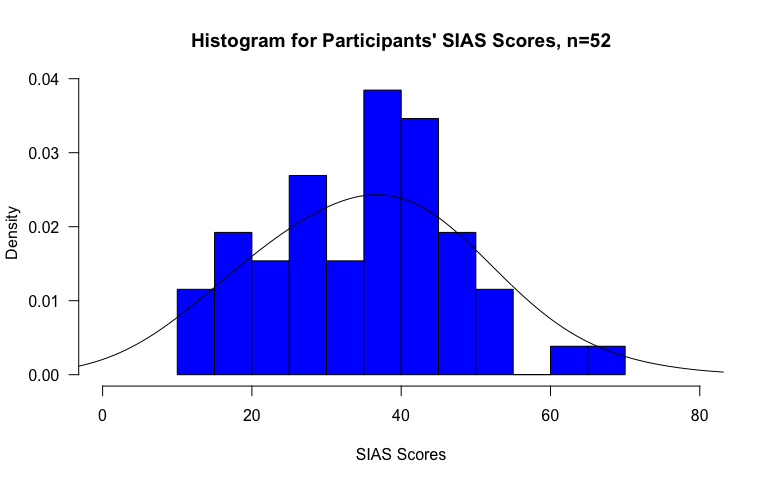
\includegraphics[width=0.6\textwidth]{./figures/sias_distri_52.png}
\caption{The distribution of SIAS scores for recruited participants}
 \label{fig:sias}
\end{figure}

Along with pre-assessment, we explained the study to each participant before receiving consent. Then, we installed a custom mobile app, Sensus~\cite{sensus, sensus-paper}, on each participant's personal smartphone. Participants were informed that the application passively collected the GPS location information every 150 seconds and accelerometer data every second (1Hz), then uploaded it to an Amazon Web Services S3 server.
%When the experiment was completed, all participants' anonymized raw data was available for analysis.

%Yu: briefly introduce what is and how to answer the research questions 
\subsection{Understanding Behavioral Dynamics of Social Anxiety} 
We are interested in three primary research questions in this work: 
\begin{enumerate}
\item Can we identify behavioral patterns that occur around social interactions that vary as a function of social anxiety level?
\item Do these behavioral patterns differ across communication media?
\item Do these behavioral patterns vary across different semantic locations?
\end{enumerate}
To address these questions, we model the smartphone as a linear dynamical system with the accelerometer data as the output. We then use the stimuli of the system to extract hidden patterns of human behavior around the time social interactions occur.  In this paper, we consider phone calls and text messages made or received by participants to be representative social interactions.

\section{Approach for Modeling Behavioral Dynamics}
\label{sec:approach}
% I have re-written this section--Yu
% Be careful with your edits here: if you want to edit terms, please add comment starting with "FIXME"--I used some terms in figures too so I need to know if any of needs to be changed.---Yu

\label{approach}
% I have re-written this paragraph--Yu
In this section, we discuss the approach for the proposed study.  Figure~\ref{fig:diagram} illustrates the data structure and framework of our methodology for learning behavioral dynamics.  We first collect GPS data, accelerometer data, and communication events (i.e., phone calls and text messages). Next, we pre-process this data by aligning observations all temporally.  The accelerometer data consists of three dimensions (X, Y, and Z axes), and the communication event data includes the time and duration of a phone call or text message. The raw GPS data is transformed into semantic locations that integrate its social context. After structuring all the data, we use a sliding window to isolate periods of time before, during, and after each phone call or text message.  Next, by modeling the smartphone as a linear dynamic system, the three-dimensional accelerometer data in all the sliding windows belonging to a single call or text message is reduced to a one-dimensional system stimulus. Finally, we construct a distance matrix using the histogram distribution of the system stimulus and combine this with the GPS semantic labels for further analysis.  These distance matrices allow us to characterize the behavioral dynamics of a participant before, during, and after a phone call or text message.


% should I use [X Y Z] or y(t) in the caption? --Yu
\begin{figure}[htbp!]
\centering
\includegraphics[width=1.0\textwidth]{./figures/diagram_framework_3.png}
\caption{Study framework: The top portion of this image shows an example of the data and the sliding window used to segment it. The three-dimensional accelerometer data ($X,Y,Z$) are aligned together with smartphone communication data (phone calls and text messages) and semantic GPS locations temporally. For the GPS locations, green represents food and leisure places, brown represents work places, blue represents home, yellow represents personal life locations, and purple represents a transition between places. The bottom portion shows the feature extraction method: After being segmented into sliding windows and dimensionality reduction through the linear dynamic model, the three-dimensional accelerometer data, $y(t)$, is reduced to a one-dimensional system stimulus, $u(t)$. Each phone call and text is represented by features extracted from distance matrices that contain Euclidean distances between pairs of histogram distributions of the one-dimensional system stimulus.}
 \label{fig:diagram}
\end{figure}

%Comments for Yu: Please change "Histogram of Us" to "Histogram of Motion Stimulus"-done

\subsection{Preprocessing}
There are several steps taken to preprocess our data in order to build the linear dynamical system and perform unsupervised feature learning: 

\begin{enumerate}
\item Label raw GPS data with social semantics (e.g., ``food and leisure'' if a GPS location corresponds to a restaurant). 
\item Segment time period around a phone call or text message into sliding windows.
\item Retrieve the accelerometer data in each window to capture motion information for specific phone calls or text messages. 
\end{enumerate}

\subsubsection{GPS Data}
To acquire the location semantics for GPS trajectory data for each individual, we first cluster the GPS trajectories by spatial and temporal locality~\citep{kang2004extracting,huang2016assessing}. Then, we use the Foursquare Location-Based Social Network to obtain Point-of-Interest (POI) information (e.g., residence area, academic building, and restaurants) for each location cluster. Further, we group all of the clusters using five types of location labels:

\begin{itemize}
\item \textbf{Work:} For the college students in this study, work locations are mostly within the campus, but dormitories are excluded.
\item \textbf{Food \& Leisure:} This location set includes restaurants, bars, clubs and shopping centers. 
\item \textbf{Home:} Some participants have multiple home locations. In this study, we do not distinguish between them.
\item \textbf{Transition:}  This includes all the time the participants spent on transit (walking, driving etc).
\item \textbf{Personal Life:}  Locations that do not belong to the previous categories, such as post office, grocery store, etc.
\end{itemize}

The labels extracted from GPS data confer semantic location information to provide deeper contextual meaning about the  interaction between behaviors, locations, and social anxiety levels.  Additionally, the labels help identify potential locations where interventions might be needed.

\subsubsection{Communication Events}
\label{communicationEvent}
% In any event, we shouldn't put this paragraph here, maybe in introduction and design of study.---Yu

% To learn the behavior dynamics of smartphone use, the proposed data processing framework focuses on the behavior data around the events that are related to cell phone use. Regarding social anxiety, the significant behaviors of cell phone use contains call and text. Therefore, the timing information of contacts data recorded by the \textbf{Sensus}\textit{(we redact the name of the app for anonyminity elsewhere should we here too?MR)}  application is used to identify the moments of smartphone use.

In our study, communication events refer to phone calls and text messages. As discussed in Section~\ref{intro}, previous research in psychology has demonstrated that smartphone communication patterns and behaviors are related to social anxiety.
To capture the behaviors around those communication events for a better understanding of the relationship between social anxiety and behavioral dynamics, we first define the observation period for a communication event: $\alpha_{1}$ minutes before and after a communication event (and its duration if it is a phone call).  Our choice of the observation period is based on the anticipated impact of social anxiety on behavioral dynamics. For instance, a subject might hesitate for a period before calling an important person or struggle when no one answers her call. The observation period also determines the settings of accelerometer data in Section~\ref{accdata}.%%LEB:  I dont understand what you mean by settings of the accelerometer data-- --we get acc falling in the same window-Yu

\subsubsection{Accelerometer Data}
\label{accdata}
After defining the observation period in Section~\ref{communicationEvent}, we use the accelerometer data within that time period to analyze the behavioral dynamics.  Figure~\ref{fig:29min_call} gives an example of a 29-minute accelerometer data session that captures the motions of the smartphone when the subject makes a 9-minute phone call. In this example, $\alpha_{1}=10$ minutes.
Before conducting further analysis of behavioral dynamics of a communication event using the accelerometer data in the observation period, we will first apply a sliding window process to segment the observation period and the accelerometer data in it into smaller, fixed-size chunks. Section~\ref{feature for acc} describes this in more detail.


%Yu, please insert a figure here.--done, 29-min phone call window (call is 9min)

\begin{figure}[htbp]
\centering
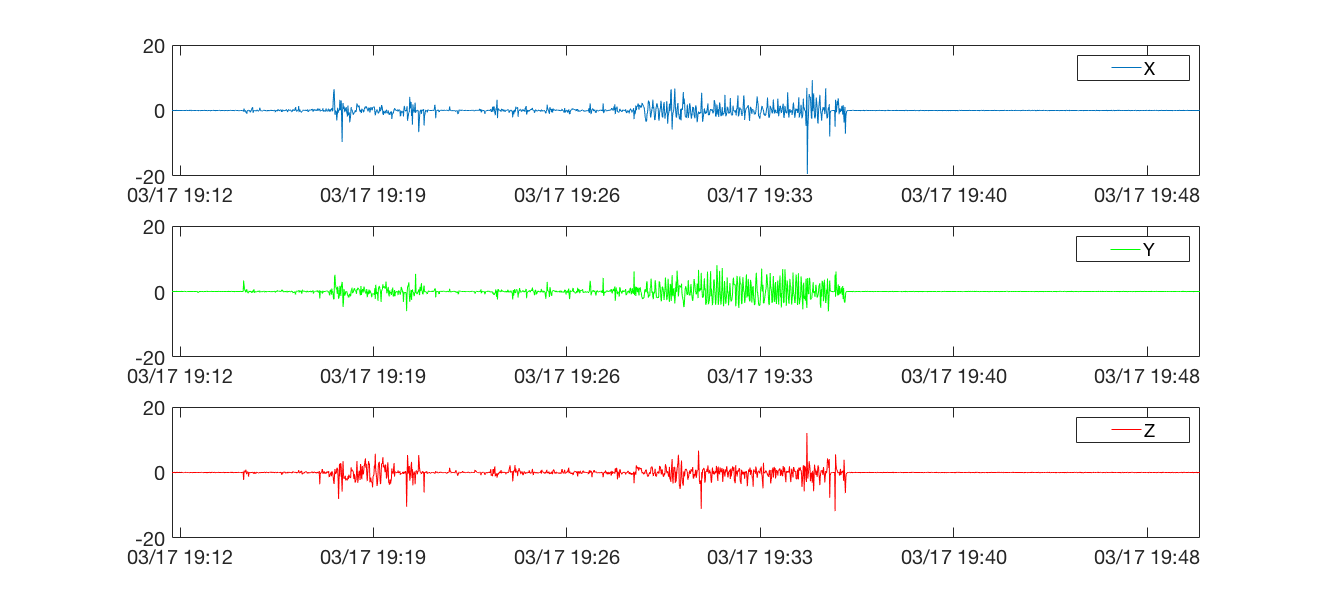
\includegraphics[width=0.7\textwidth]{./figures/29_min_call.png}
\caption{The accelerometer data for a 29-min phone call}
 \label{fig:29min_call}
\end{figure}



%Need to rewrite this section--Yu
\subsection{Mathematical Formulation}
\label{mathform}
In this section, we present the mathematical formulation of the proposed framework shown in Figure~\ref{fig:diagram}. For individual $i$, all the observed behavioral data $X(i)$ can be represented as: 

\begin{equation}
X(i)=\{[AC(i)(1),LC(i)(1), LG(i)(1)], \cdots,[AC(i)(j),LC(i)(j), LG(i)(j)],\cdots, [AC(i)(m),LC(i)(m), LG(i)(m)]\}
\end{equation}
%FIXME would it make more sense for i to be a subscript? Also, below it sounds like our windows are of varying sizes based on the length of calls. Is this a change we made for the distance matrix? I don't remember this being how we formulated the now no longer used t-SNE processing. MR

$AC(i)(j)$ represents the accelerometer data in the observation period $j$, which also corresponds to the specific communication event $LC(i)(j)\in \{\mathrm{`Call'}, \mathrm{`Text'}\}$.  As described in Section~\ref{communicationEvent}, the period length is: $2*\alpha_{1} + \mathrm{DurationOfCommunicationEvent}$. %(we consider $DurationOfCommunicationEven = 0$ if $LC(i)(j)='Text'$).
$m$ is the total number of the communication events for individual $i$, including phone calls and text messages.
 $LG(i)(j)\in \{`Home',`Work',`Food \& Leisure',`Transition',`Personal Life'\}$ represents the GPS label in the observation period $j$.

Since this study aims at understanding the relationship between behavioral dynamics of smartphone use and social anxiety, the goal of the proposed learning framework is to extract metrics and features from the observed behavior data and analyze the correlations between these features and the SIAS score, $SIAS(i)$. Using $FAC(i)(j)$ to represent a feature extracted from the accelerometer data of the observation period $j$, AC(i)(j), a metric example that represents behavioral dynamics of a phone call event for individual $i$ is represented as:

\begin{equation}
\label{MC}
MC(i)=\overline{FAC(i)(j)} \qquad \{j: LC(i)(j) == `Call'\} 
\end{equation}

%FIXME: I feel like we could really clean up the math notation. Something like... (MR)
%\(\phi: \text{AC} \mapsto \mathbb{R}\)
%\(\text{AC}_i^c = \{(x,y,z) : (x,y,z) \in \text{AC}_i(j) \cap \text{LC}_i(j) \not= \text{Other} \ \forall j \}\)
%\(\text{MC_i} = \overline{\phi(\text{AC}_i^c)} \)


The metric~\ref{MC} refers to the average value of the features extracted from the accelerometer data that belongs to the observation period $j$ of individual $i$. Similarly, an example that represents behavioral dynamics of individual $i$ of a text event can be represented as:

\begin{equation}
\label{MT}
MT(i)=\overline{FAC(i)(j)} \qquad \{j: LC(i)(j) == `Text'\}
\end{equation}

The metric~\ref{MT} is the average value of the features extracted from the accelerometer data  that belongs to the observation period $j$ of individual $i$ during a text event.

Based upon previous work on self-reported behavioral preferences of socially anxious subjects~\cite{reid2007text} and the greater social demands of typical phone calls relative to text messages~\cite{reid2004insights}, we hypothesize that the impact of social anxiety on behavioral dynamics of phone call events should be higher than the impact on text events. In other words, we anticipate that the correlation between $MC(i)$ and $SIAS(i)$ should be higher than the correlation between $MT(i)$ and $SIAS(i)$. The goal of our study is to validate this in-lab conclusion in a natural environment with a micro-level motion analysis.

%, which can provide evidence and methodology for future real-time monitoring and intervention.% did we mention monitoring before?I just wrote it here for now--Yu
% Yes kjl

\subsection{Feature Extraction from Accelerometer Data}
\label{feature for acc}

In this section, we introduce the details of the feature extraction of accelerometer data through the linear dynamic model. Specifically, we discuss the process to calculate $FAC(i)(j)$, which represents the feature extracted from the accelerometer data of the observation period $j$, $AC(i)(j)$.

\subsubsection{Sliding Windows of Accelerometer Data}
As introduced in Section~\ref{mathform}, $AC(i)(j)$ represents the accelerometer data in the observation period $j$ for individual $i$, which corresponds to a specific communication event $LC(i)(j)\in \{`Call', `Text'\}$. To begin extracting the features of behavioral dynamics from $AC(i)(j)$, we first segment it with sliding windows.  Recall that each observation period spans several minutes (depending on the value of $\alpha_{1}$).  Essentially, we consider multiple small fixed-size windows over the length of the observation period. 
%\textit{(doesn't \(j\) represent the segmentation already? Do we need to say that we being by segmenting AC(i)(j)? MR)}.---------------No, here j refers to an entire period of a event, Yu

We use $\alpha_{2}$ to represent the length of a single sliding window, and $\alpha_{3}$ to represent the stride or offset of each window into the observation period.
%We need to explain 'stride' here, I gave up on how to make it clear in english----Yu
For example, the accelerometer data of the observation period in Figure~\ref{fig:29min_call} for the 9-minute call is segmented as 20 sliding windows, each of which has 10 minutes of accelerometer data when $\alpha_{2}$=10 minutes and $\alpha_{3}$=1 minute. Therefore, $AC(i)(j)$ is segmented into data pieces, each of which has a fixed-size length.  Each window can be represented as:

\begin{equation}
\label{AC series}
AC(i)(j)=\{AC(i)(j)(1),\cdots, AC(i)(j)(k), \cdots, AC(i)(j)(n)\}
\end{equation}

Where $AC(i)(j)(k)$ represents the accelerometer data of the $k^{th}$ sliding window of the observation period $j$ (and also the corresponding communication event) of individual $i$, and the sample length of the accelerometer data $AC(i)(j)(k)$ is $\alpha_{2} \times \mathrm{SamplingRateOfAccelerometerSensor}$. The dimension of $AC(i)(j)(k)$ is $3 \times \alpha_{2} \times \mathrm{SamplingRateOfAccelerometerSensor}$ due to the nature of accelerometer data. After segmenting the accelerometer data into sliding windows, we reduce the dimensionality of the accelerometer data $AC(i)(j)(k)$ to generate features to characterize behavioral dynamics.% or 'variations'? or "characteristics" of behavior dynamics ? ----Yu

\subsubsection{Dimensionality Reduction through Linear Dynamical Model}

After data preprocessing and segmentation, the raw time-series accelerometer data for a single communication event $AC(i)(j)$ has been segmented into data pieces (see Equation~\ref{AC series}) by using sliding windows. Each data piece has identical dimensionality. Here, we adopt a model-driven technique~\cite{gong2016piecewise} to reduce the dimensionality of the data piece $AC(i)(j)(k)$ from $3 \times \alpha_2$ to a chosen value $x$.\footnote{$x$ refers to the number of bins used when quantizing the accelerometer data.  For this paper, we chose $x=11$.}  With $\alpha_2=10$ minutes and our chosen value $x=11$, we reduced dimensionality from $3 \times 600$ to $11$.

% Edited KL
% OK, someone, please edit this paragraph based on the basic claim below, I don't know how to make it readable and convincing.--Yu
%The basic claim here is: moods can be implied by behaviors, and behaviors are raised/affected by events. Thus, something of events triggered behaviors. In this case, some hidden magic(system stimuli) generates human behavior(accelerometer data we observe), so let's use the magical thing as a feature ---Yu 
We view smartphones as dynamical systems based upon our novel application of prior art.  Ekkekakis \emph{et al.}~\cite{ekkekakis2013measurement} discussed how mood affects one's appraisal of a situational event.  In our study, social anxiety is a mood-related measure, and each communication event is a situational event.  Accordingly, the behavioral dynamics of phone usage are appraisals of these communications events.  Thus, a socially anxious individual will produce behavioral dynamics consistent with her anxiety, stimulating the accelerometer sensor to generate rich information. 
% * <bat5x@virginia.edu> 2017-02-15T19:24:08.993Z:
% 
% > novel application of prior art
% prior art? not clear
% 
% ^.

%Inspired by the state-of-the-art studies that have provided model-driven techniques based on the knowledge of human behavioral dynamics of cell phone use~\cite{ekkekakis2013measurement},
%we hypothesize that human moods facilitate appraisals of situational events in a way that is consistent with the mood.% I don't know what this sentence means....--Yu
%In our study, social anxiety level is a mood-related measure, % can you say it's mood-related measure? --Yu
%and the communication events of cell phones are situational events. Accordingly, the behavioral dynamics of cell phone use are appraisals of the communications events of cell phones.
%Further, it can be explained that when socially anxious individual operates on the cell phone, his anxiety will facilitate motion dynamics that are consistent with his anxiety. These anxious motion dynamics will stimulate the accelerometer sensor of the cell phone to generate data with rich information.


Thus, we propose that a smartphone can be viewed as a dynamical system that the subject operates with stimuli caused by social anxiety level. Using this analogy, the human can be viewed as a control system, while the smartphone is an observer system with certain states, and the accelerometer is the measurement system. The salient information is the motion stimuli that are highly related to the behavioral dynamics caused by the social anxiety of each subject. Therefore, we adjust a linear dynamical model to estimate the motion stimulus of the accelerometer data.



The proposed linear dynamic model is described as follows:
\begin{equation}
\label{lds}
\begin{cases}
  \parallel u(\bullet)\parallel_{\iota 0}  \leq  k  \\
  |u(t)| \leq 1 \qquad \forall t  \\
  \Sigma_{t} \parallel CA^{t}B \parallel_{1} \leq \mu  \\
  x(t+1) = Ax(t)+Bu(t)\\
  y(t)=Cx(t) + N
\end{cases}
\end{equation}

In this model, we use $y\in R^{3 \times T}$ to represent the data piece, $AC(i)(j)(k)$, while $T = \alpha_{2} \times$ SamplingRateOfAccelerometerSensor. Also, we use $y(t)\in R^{3 \times 1}$ to represent the accelerometer data at  time $t$. Thus, based on the insight of modeling smartphone as a dynamical system, $y(t)\in R^{3}$ is the output of the linear dynamical system (the smartphone) driven by a one-dimension sparse and bounded stimulus, $u(t)\in R$. The dynamical system for estimating the motion stimulus includes two parts: the linear state space transition, the fourth line in Equation~0\ref{lds}, and linear observation, the fifth line in Equation~\ref{lds}.
The linear state space transition is defined by a system matrix $A \in R^{p \times p}$, a stimulus matrix $B \in R^{p \times 1}$ and a system state vector, $x(t) \in R^{p \times 1}$. The linear observation is defined by an observation matrix $C \in R^{3 \times p}$ and the probability $N \in R^{3 \times 1}$ of the random noise. In the above definition, $p$ represents the system order of this linear dynamic model, which determines the complexity  of the model.
The dimension of the observation  $y(t)$ is $3 \times 1$, because the accelerometer data is 3-axis data.
$\parallel u(\bullet)\parallel_{\iota 0} $ is the number of nonzero elements in the stimulus sequence. 

An expectation-maximization (EM) algorithm is applied to estimate the $A$, $B$, $C$, $S$, and $u$ with the assumption of system linearity and time invariance. Although the observation matrix $C$, which is related to the accelerometer sensor, depends on the physical characteristics of the sensor, and the probability function of random noise $N$ depends on the noise characteristics of the accelerometer sensor, we make a simplified assumption that both of them are linear and time-invariant.

After the EM algorithm, we estimate the system motion stimulus, $u$, of the accelerometer data piece $y$. Here $u$ has a dimension of $1 \times T$. To construct a feature to represent $y$, we extract the histogram of the stimulus vector $u$, $h(u)$. Each histogram is quantized into 11 bins, equally spaced in a range from -1 to 1. Until now, the previous high-dimension accelerometer data piece is reduced to $1\times 11$ dimensions. This 11-dimension feature can be represented as $HU(i)(j)(k)$, that is extracted from $AC(i)(j)(k)$.

\subsubsection{Metrics for Accelerometer Data of a Communication Event} % can we have a better subtitle? --Yu

After dimensionality reduction through the linear dynamic model, the raw high-dimension accelerometer data of a communication event, $AC(i)(j)(k)$, can be represented as a series of low-dimension features:

\begin{equation}
\label{HU series}
AC(i)(j)=\{HU(i)(j)(1),\cdots, HU(i)(j)(k), \cdots, HU(i)(j)(n)\}
\end{equation}

Next, we develop features to capture the behavioral dynamics of a communication event $AC(i)(j)$. State-of-the-art work has explored metrics of feature arrays including statistical features~\cite{bishop2006pattern}, autoregressive modeling~\cite{sapankevych2009time}, and singular value decomposition~\cite{liu2013modeling}. Since our work is the first attempt to explore the behavioral dynamics and analyze the relationship with social anxiety levels, we simplify the process by adopting statistical features.

We want the extracted features to be capable of indicating the characteristics of motions around a communication event. For example, if a subject is very anxious when she makes a phone call, her hand may shake more than usual or she may pace around with the phone.  The features should be able to capture such anxiety-related motion. Thus, we generate features that can show the variations of the motions by first creating a distance matrix, $DM$, that calculates the similarity between pairs of $HU(i)(j)(k)$ of a communication event, $AC(i)(j)$. Each element of the distance matrix $DM(i)(j)$ is the Euclidean distance between the pairs of the 11-dimensional features, $HU(i)(j)(k)$:
%FIXME: Maybe I don't know what "statistical features" are, but isn't that just a generic term for things like average, min, max, variance etc... of a set? Why would our first step to generate features be creating a distance matrix? I guess this probably is in line with your comment above too about multiple uses of 'features'? I'm probably misunderstanding something. MR---My guess is, anything we extract in the process of learning can be called features...Not sure though ---Yu

\begin{equation}
DM(i)(j)(a)(b)= Distance[HU(i)(j)(a), HU(i)(j)(b)] \qquad a,b \in \{1 \cdots n\}
\end{equation}

Then, we use the mean value and standard deviation of the distance matrix $DM(i)(j)$ as the metrics of a communication event  $AC(i)(j)$. 
Thus, now the accelerometer data of $AC(i)(j)$ generates two metrics, corresponding to the representation in Equations~\ref{MC} and~\ref{MT}, $FAC_1(i)(j)$ and $FAC_2(i)(j)$ refer to the mean value and standard deviation of $DM$, respectively:

\begin{equation}
FAC_1(i)(j)=\overline{DM(i)(j)}
\end{equation}
\begin{equation}
FAC_2(i)(j)=std(DM(i)(j))
\end{equation}

In summary, after preprocessing and applying linear dynamic model, we are able to reduce the high-dimensional raw temporal motion data to a low-dimensional feature array. These arrays are considered pairwise to construct a distance matrix which uniquely characterizes each subject's behavioral dynamics during smartphone use. Then, we develop the statistical features for communication events for further analysis.



\section{Analysis and Results}
\label{sec:results}
In this section, we present the analysis and results of our study. We first summarize the features used for unsupervised learning, and then the relevant parameters for further exploration of the relationship between social anxiety status (measured by SIAS score) and behavioral dynamics. 

%After the feature extraction, we used the Pearson correlation and significance analysis between social anxiety status and the smartphone use, including both phone calls and text messages.  Last, we analyzed the effect size between high and low social anxiety groups considering the behavioral dynamics to explore the difference between them.
%FIXME: I feel like the sequence of events here isn't clear. I think it feels like we go from analysis  ("We first...") to methodology ("In this study, after the feature extraction,..."). MR  %agreed KL

\subsection{Summary of Features and Parameters}
\label{features_and_parameters}
As discussed in Section~\ref{approach}, we extract features from the motion information during phone calls and text messages along with GPS semantic information.  We also define the parameters used for the analysis in this paper.

\subsubsection{Features for Analysis}
We also develop features from the percentage of phone calls and text messages at different GPS locations. All the features we use in the analysis and their explanations are listed in Table~\ref{tab:def}.

% \begin{enumerate}
% \item Proportions of phone calls made at different GPS semantic locations
% \item Proportions of texts made at different GPS semantic locations
% \item \label{avg_mean_call} The mean value of all distance matrices' mean ($\overline{DM}$) that describes the motions of all the phone calls one participant made
% \item  \label{avg_std_call} The mean value of all distance matrices' standard deviation ($std(DM)$) that represents all the phone calls one participant made
% \item  \label{avg_mean_text} The mean value of all distance matrices' mean ($\overline{DM}$) that describes the motions of all the text messages one participant made
% \item  \label{avg_std_text} The mean value of all distance matrices' standard deviation ($std(DM)$) that represents all the text messages one participant made
% \item The mean value of all distance matrices' mean ($\overline{DM}$) that describes the motions of the phone calls one participant made at different GPS semantic locations
% \item The mean value of all distance matrices' standard deviation ($std(DM)$) that represents the phone calls one participant made at different locations
% \item The mean value of all distance matrices' mean ($\overline{DM}$) that describes the motions of the text messages one participant made at different GPS semantic locations
% \item The mean value of all distance matrices' standard deviation ($std(DM)$) that represents the text messages one participant made at different locations
% \end{enumerate}




\begin{table}
\caption{Terms used for features and the definitions. \label{tab:def}}
\begin{center}
\small
%\def\arraystretch{1.5}
	\begin{tabular}{ c  p{5in} }
    \toprule
    			\textbf{Term}				&   	\textbf{Definition}			\\
        \midrule
        $Call\_Proportion$				&	The proportions of phone calls at different locations\\
        $Text\_Proportion$				&	The proportions of text messages at different locations\\
        $\overline{FAC_1}$				&	The average of the mean values of all distance matrices ($DM(i)$) belonging to a subject \\  
        $\overline{FAC_2}$				&	The average of the standard deviations of all distance matrices ($DM(i)$) belonging to a subject\\
        $MC$				&	The metric for a phone call event\\
        $MT$				&	The metric for a text message event\\
        \bottomrule
	\end{tabular}
\end{center}
\end{table}


These six features are extracted from the raw data we collected from the participants with linear dynamic model and the distance matrix described in Section~\ref{approach}. They are used to further explore the relationship between behavioral dynamics and social anxiety status together with the study parameters. 


\subsubsection{Parameters for Relationship Exploration between Mental State and Behavior}
\label{parameters}

% table2: pearson correlation--- call and text matrix features without location info

\begin{table*}
\caption{Correlation and Significance Analysis of motion data  around phone calls and text messages vs. SIAS Score: Pearson Correlation (with p-values) between participants' SIAS Scores and the features extracted from the smartphone accelerometer data around phone calls and texts. In this table, two features are explored: 1) the average of all distance matrices mean ($\overline{FAC_1}$), and 2) the average of all distance matrices standard deviation ($\overline{FAC_2}$).
\label{tab:pearson_matrix_call_text}}
\begin{center}
\small
\def\arraystretch{1.5}
	\begin{tabular}{ l @{\hskip 0.5in} r r r r r}
    \toprule
											& \multicolumn{2}{c}{Call (MC)} 							&	& \multicolumn{2}{c}{Text (MT)} \\
        \cline{2-3} \cline{5-6}
    	Matrix feature						& Pearson r					& p-value				&	& Pearson r				& p-value		\\
        \hline
        $\overline{FAC_1}$						& \textbf{0.2867}					& \textbf{0.0457}				&	& 0.1961					& 0.1634		\\
        $\overline{FAC_2}$						&\textbf{ 0.3041}					& \textbf{0.0336}				&	& 0.2342				& 0.0946		\\
        \bottomrule
	\end{tabular}
\end{center}
\end{table*}

\begin{figure*}
\begin{center}
    \begin{subfigure}[b]{.24\textwidth}
        \includegraphics[width=\textwidth]{./figures/fig-corrplot-mc-1.pdf}
        \caption{$r=0.2867$.}
    \end{subfigure}
    \begin{subfigure}[b]{.24\textwidth}
        \includegraphics[width=\textwidth]{./figures/fig-corrplot-mc-2.pdf}
        \caption{$r=0.3041$.}
    \end{subfigure}
    \begin{subfigure}[b]{.24\textwidth}
        \includegraphics[width=\textwidth]{./figures/fig-corrplot-mt-1.pdf}
        \caption{$r=0.1961$.}
    \end{subfigure}
    \begin{subfigure}[b]{.24\textwidth}
        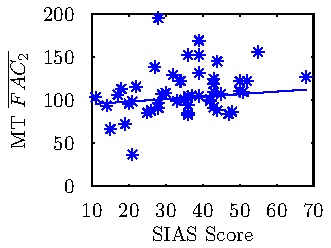
\includegraphics[width=\textwidth]{./figures/fig-corrplot-mt-2.pdf}
        \caption{$r=0.2342$.}
    \end{subfigure}

%    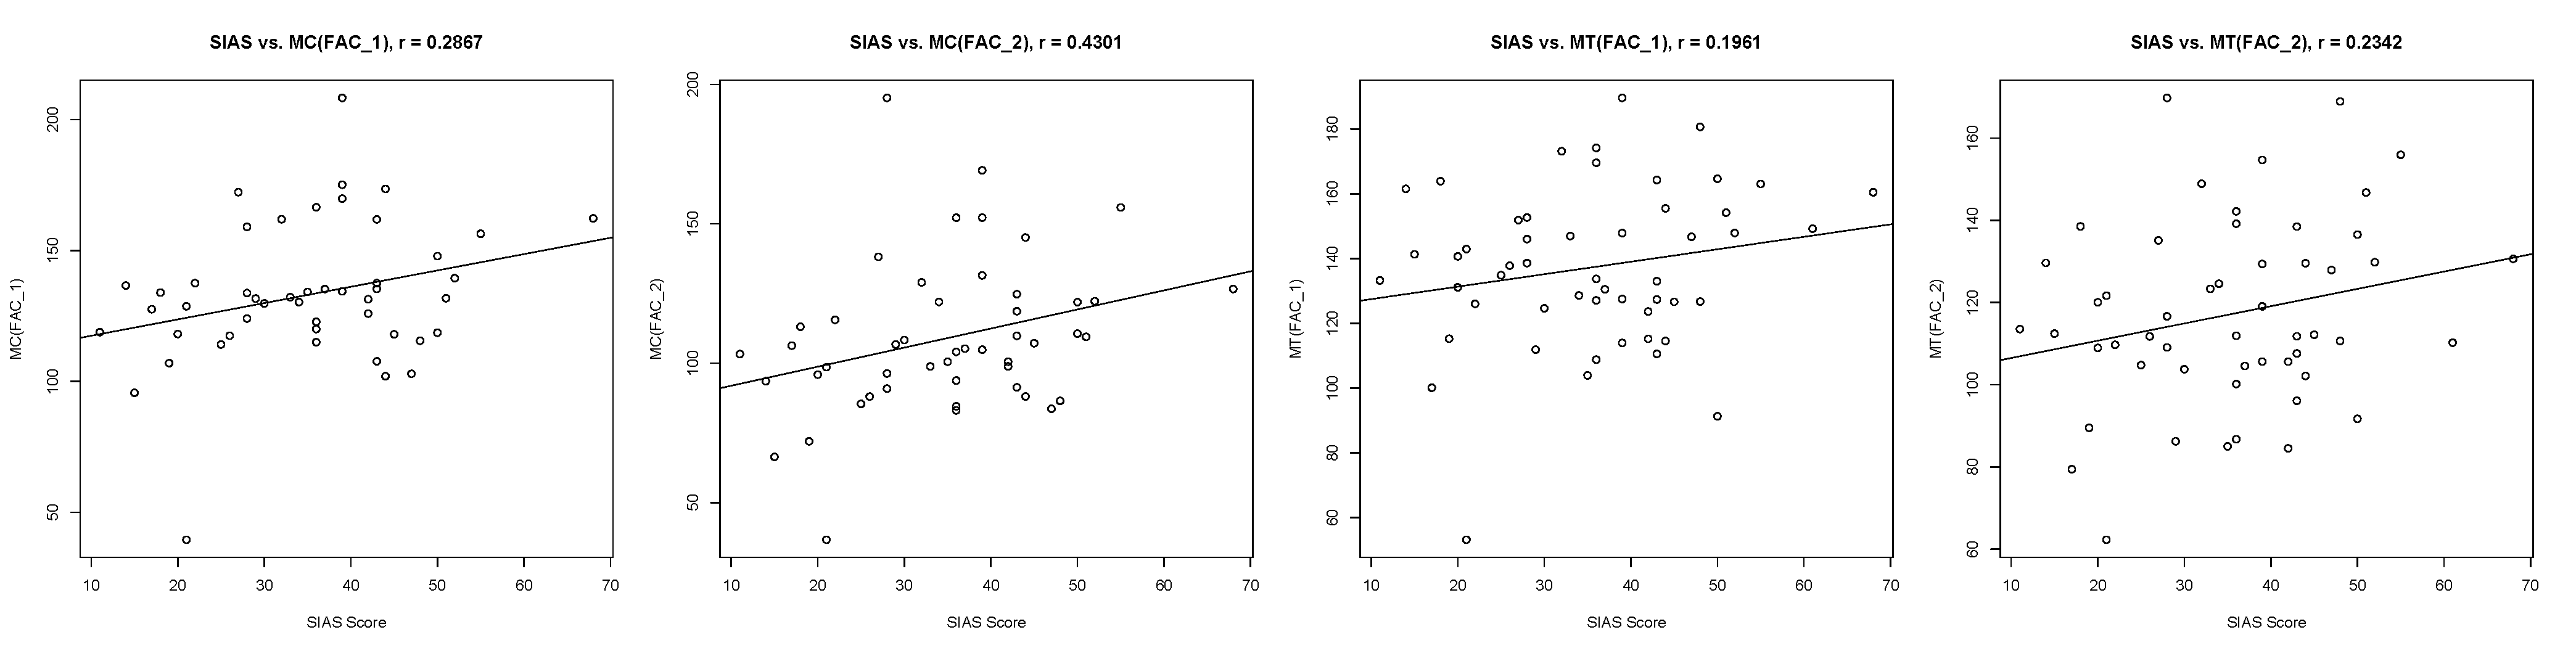
\includegraphics[width=\textwidth]{./figures/corrplot.pdf}
    \caption{Correlation plots of SIAS score vs. matrix
    features (cf. Table~\ref{tab:pearson_matrix_call_text}).\label{fig:corr}}
\end{center}
\end{figure*}




For further analysis, we define two parameters for the study:
\begin{enumerate}
\item GPS locations: we conduct an analysis exploring the relationship with and without GPS semantic information to understand the effect of locations on social context. 

\item Grouping of the participants: according to the SIAS measure of all participants, we group the participants in two different ways to analyze the effect size: 
% * <bat5x@virginia.edu> 2017-02-15T19:32:56.562Z:
% 
% can you clarify what cutpoints used & why those were selected for both the 2 & 3 group approaches
% --- cut points are introduced in 'results' part.--Yu
% ^ <bat5x@virginia.edu> 2017-02-15T22:12:19.105Z:
%
% I don't see the cutpoints for 2-group approach - refers back to this section 
%
% ^.
	\begin{itemize}
		\item  Two-group setting: we use one SIAS threshold to divide the participants into two groups, and then we compute the effect size between the two groups. This setting provides a general division of our participants.
		\item  Three-group setting: we use a low SIAS and a high SIAS threshold to split the participants into three groups: 1) low social anxiety risk, 2) medium social anxiety risk, and 3) high social anxiety risk.   We analyze the effect size  between the low social anxiety risk group and the high social anxiety risk group. This setting provides a more distinguished grouping of the participants.
	\end{itemize}
\end{enumerate}






\begin{table}[b]
\caption{Correlation and Significance Analysis of proportions of phone calls made at different locations vs. SIAS Score: Pearson Correlation (with p-values) between participants' SIAS Scores and the portions of phone calls that were made in specific types of locations.  Additionally, the normalized mean  ($\bar{x}$) and standard deviation ($\sigma$) of participants' portions of phone calls at each location are shown.\label{tab:pearson_call_text}}
% * <bat5x@virginia.edu> 2017-02-15T21:01:12.020Z:
% 
% > with p-values) 
%  unclear why some p-values <.05 are bolded (for home), but not others (personal life  - texts)
% 
% ^.
%---This is good point...should we also talk about it? Yu
\begin{center}
\small
\def\arraystretch{1.5}
	\begin{tabular}{ l @{\hskip 0.5in} r r r r r r r r r }
    \toprule   % I added the top/bottomrule----Yu
                  				& \multicolumn{4}{c}{Call\_Proportion} 														&	& \multicolumn{4}{c}{Text\_Proportion} \\
        \cline{2-5} \cline{7-10}                        
    	Location 				& Pearson r 		& p-value 			& $\bar{x}$ 		& $\sigma$ 			&	& Pearson r 		& p-value 			& $\bar{x}$ 		& $\sigma$ 	\\
		\hline
        Work 					& -0.1806			& 0.2142  			& 0.0935			& 0.1074			&	& -0.2511			& 0.0725			& 0.1441 			& 0.1040  			\\
        Home 			& \textbf{0.3983} 	& \textbf{0.0045} 	& 0.3868 	& 0.2484	&	& \textbf{0.4059}	& \textbf{0.0028}	& 0.3989	& 0.2128	\\
        {Food \& leisure} 		& -0.2342 			& 0.1053 			& 0.1188 			& 0.1551			&	& -0.0882			& 0.5340			& 0.1412			& 0.1423 			\\
        Personal life 			&	0.1234 			& 0.3982 			& 0.0138 			& 0.0346			&	& \textbf{-0.2917}			& \textbf{0.0359}			& 0.0166			& 0.0228 			\\
        Transition 				& -0.0715 			& 0.6141 			& 0.3200 			& 0.1812			&	& -0.0707			& 0.6045			& 0.2381			& 0.1153 			\\
        \bottomrule
  	\end{tabular}
\end{center}
\end{table}



% \begin{figure}[htbp]
% \centering
% 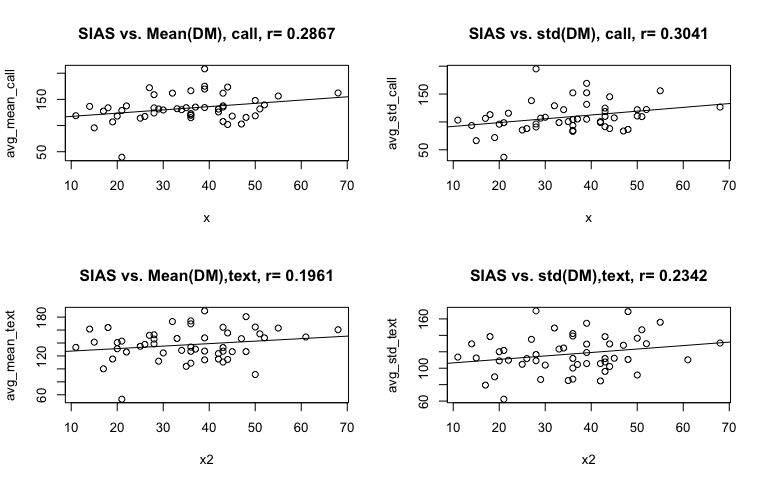
\includegraphics[width=0.5\textwidth]{./figures/corrplot.png}
% \caption{The correlation plot of SIAS vs. matrix features}
%  \label{fig:corr}
% \end{figure}






% table3: pearson correlation--- call and text matrix features with location info
\begin{table}[b]
\caption{Correlation and Significance Analysis of motion data around phone calls and text messages at different locations vs. SIAS Score: Pearson Correlation (with p-values) between participants' SIAS Scores and the features extracted from the smartphone accelerometer data around phone calls and text messages at different locations. In this table, two features are explored: 1) the average of all distance matrices mean ($\overline{FAC_1}$), and 2) the average of all distance matrices standard deviation ($\overline{FAC_2}$).
\label{tab:pearson_matrix_call_text_GPS}}
\begin{center}
\small
\def\arraystretch{1.5}
	\begin{tabular}{ l @{\hskip 0.5in} r r r r r r r r r r r}
    \toprule
									& \multicolumn{5}{c}{Call (MC)}																		&	& \multicolumn{5}{c}{Text (MT)} \\
        \cline{2-6} \cline{8-12}
        							& \multicolumn{2}{c}{$\overline{FAC_1}$} 			&	& \multicolumn{2}{c}{$\overline{FAC_2}$}			&	& \multicolumn{2}{c}{$\overline{FAC_1}$} 	&	& \multicolumn{2}{c}{$\overline{FAC_2}$}	\\
        \cline{2-3} \cline{5-6} \cline{8-9} \cline{11-12}
    	Location					& Pearson r			& p-value					&	& Pearson r			& p-value				&	& Pearson r			& p-value					&	& Pearson r			& p-value			\\
        \hline
        Work						& -0.1204			& 0.5115					&	& 0.0477			& 0.7954				&	& -0.2107			& 0.1461					&	& -0.1192			& 0.4148			\\
         Home				       & 0.1066	                & 0.4858			    &	& 0.2083	        & 0.1697		&	& 0.1586	& 0.2712			&	& 0.2242	& 0.1174	\\
        \textbf{Food \& leisure}			& \textbf{0.3679}			& \textbf{0.0323}					&	&\textbf{ 0.446}			& \textbf{0.0082}				&	& 0.1591			& 0.2800					&	& 0.2181			& 0.1365			\\
        Personal life				& -0.331			& 0.3502					&	& -0.3531			& 0.3169				&	& -0.0532			& 0.7760					&	& -0.0345			& 0.8539			\\
        Transition					& 0.2204			& 0.1364					&	& 0.2503			& 0.0896				&	& 0.1382			& 0.3333					&	& 0.1395			& 0.1183			\\
	\bottomrule
    \end{tabular}
\end{center}
\end{table}


\subsection{Correlation Analysis}
In our study, with the features in Section~\ref{features_and_parameters}, we calculate the Pearson correlation coefficient and significance analysis to explore the relationship between human behavior of smartphone use and social anxiety status.


Table~\ref{tab:pearson_call_text} shows the Pearson correlation and significance analysis between the pre-assessed SIAS measures and the percentages of phone calls ($Call\_Proportion$) and text messages ($Text\_Proportion$) participants made in different locations. We found that  the proportions of both phone calls and text messages made at home have a significant positive relation with the SIAS score (with a p-value of $0.0045$ and $0.0028$). In other words, the higher the social anxiety level is, the more phone calls and text messages are made at home. This may suggest that people with high social anxiety prefer to make communication events at home, perhaps because they are less likely to be exposed to other people or an unfamiliar environment. In this table, the proportion of text messages in personal life locations also show a significant negative correlation with social anxiety status. 
%FIXME: should we talk about personal life here? should we highlight it?--Yu


Through the linear dynamic model, Table~\ref{tab:pearson_matrix_call_text} and Table~\ref{tab:pearson_matrix_call_text_GPS} show the Pearson correlation and significance analysis between the pre-assessed SIAS measures and the behavioral dynamics features (the mean value of $FAC_1$ and $FAC_2$ cf. Table~\ref{tab:def}).  Table~\ref{tab:pearson_matrix_call_text} describes the  correlation between participants' SIAS Scores and the feature extracted from the smartphone from the linear dynamic model when making phone calls and text messages, and the correlation plot is shown in Figure~\ref{fig:corr}. For both features, we can conclude that the motion dynamics of phone calls have a more significant positive relation with the SIAS scores (with a $p$-value of $0.0457$ and $0.0336$). Considering the definition of  $FAC_1$ and $FAC_2$, we can infer that people with higher social anxiety levels have more motion variations when they are making phone calls, but there is no significant relationship between text messaging behavioral dynamics and SIAS scores. 
% * <bat5x@virginia.edu> 2017-02-15T21:41:51.666Z:
% 
% > more significant
% isn't it the case that we can say a larger magnitude based on size of the correlation, but can't really say 'more significant' (it either is or is not significant based on the pre-established p-value being used...?
% 
% ^.
Table~\ref{tab:pearson_matrix_call_text_GPS} shows the same the analysis but with the integration of GPS semantic information. Interestingly, we can interpret these findings to suggest that higher (vs. lower) social anxiety is associated with more variation in participants' motions when making phone calls at a food or leisure location, where there is likely more opportunities for scrutiny by (unfamiliar) others. 




\subsection{Effect Size Analysis}
% * <bat5x@virginia.edu> 2017-02-15T21:49:49.264Z:
% 
% correlations are a measure of magnitude so give you an effect size so I'm not really getting what this part adds? can you clarify 
% 
% ^.
We also use effect size analysis to explore the characteristics of behavioral dynamics between low and high social anxiety groups (separately for the two-group and three-group approaches) with their GPS location semantics. In this analysis, Cohen's $d$ is used to calculate the effect size of social anxiety with locations on human behavioral dynamics. In all the tables that present the effect size analysis, results that have at least a medium effect size ($\geq 0.5$) are shown in bold typeface.

In Table~\ref{tab:cohensd_matrix_call_text}, we present the effect size analysis between low and high social anxiety groups using the mean value of $FAC_1$ and $FAC_2$. Table~\ref{two-group} uses the two-group setting we described in Section~\ref{parameters}, while Table~\ref{three-group} uses the three-group setting. Our choices for the $SIAS low$ and $SIAS high$ in  Table~\ref{three-group} are based on making the number of participants of the low and high social anxiety groups equal. The three pairs of SIAS low and high scores, $(27,44), (28,43), (30,39)$, generate a group of 15, 17, and 20 participants, respectively, for both the low and high SIAS group. In both the two-group and three-group settings, different behavioral dynamics between the low and high social anxiety groups can generally be seen during the time surrounding phone calls. This difference is more pronounced with the three-group setting in which the distributions of SIAS scores of the low and high social anxiety groups are further apart. 
% * <bat5x@virginia.edu> 2017-02-15T22:01:52.747Z:
% 
% > The three pairs of SIAS scores, $(27,44), (28,43), (30,39)$, generate a group of 15,17,20 participants respectively, for both the low and high SIAS group.
% I don't understand what these pairs refer to. Also, given: a) how small these groups are, b) they're not based on any meaningful cut points from prior literature to detail what counts as high social anxiety (so totally idiosyncratic to this unselected sample), c) we already have ES with the correlations, and d) this paper is already very long, I propose cutting this section.  
% 
% Happy to go with majority tho
% 
% ^.


Tables~\ref{tab:cohensd_matrix_call_text},~\ref{tab:cohensd_matrix_call_text_GPS_2_group},~and~\ref{tab:cohensd_matrix_call_text_GPS_3_group} summarize the effect size differences that result from not only low and high social anxiety, but also location semantics in which calls and text messages were made. Both Table~\ref{tab:cohensd_matrix_call_text_GPS_2_group} and Table~\ref{tab:cohensd_matrix_call_text_GPS_3_group} show that for locations in ``food and leisure'' and ``personal life'', there is a significant social anxiety-linked difference in behavioral dynamics on phone calls. Such an effect was also observed while in transition to these locations. 
%I think transition is fine. and it is also bold in the table. so I changed the text as below: --Yu
However, due to the uncertainty in transitions (i.e., transition periods include many kinds of environments), we will not draw strong conclusions here. 
In this analysis, all the effects were more pronounced with the three-group setting---regardless of whether the subject was calling or text messaging. Notably, call behavior effects are overall more pronounced than text message effects.  


% table5(a,b): cohen's d--- call/text's matrix features without location info

% a- two groups
%b- 3 groups
\begin{table}
\caption{Effect size analysis of the motion data around phone calls and text messages between groups with (relatively) low vs. high levels of social anxiety: In this table, two features are explored: 1) the average of all distance matrices mean ($\overline{FAC_1}$), and 2) the average of all distance matrices standard deviation ($\overline{FAC_2}$). The low and high social anxiety groups are selected in two different ways: 1) all participants are split as two groups using a SIAS threshold score, and 2) all participants are split into three groups using a low SIAS threshold and a high SIAS threshold.
\label{tab:cohensd_matrix_call_text}}
\begin{center}
\small
\def\arraystretch{1.5}
	\begin{subtable}{0.8\textwidth}
    \centering
    \begin{tabular}{ l @{\hskip 0.5in} r r r r r}    
    \toprule
    							& \multicolumn{2}{c}{Call (MC)} 						&	& \multicolumn{2}{c}{Text (MT)} \\
                                \cline{2-3}										\cline{5-6}
    	SIAS threshold			& $\overline{FAC_1}$		& $\overline{FAC_2}$			&	&$\overline{FAC_1}$		&$\overline{FAC_2}$	\\
        \hline
        23						& \textbf{0.9712}				&\textbf{ 0.9423}				&	& 0.4862				& \textbf{0.5466}			\\
        28						& \textbf{0.7769}				& \textbf{0.8486}				&	& 0.3571				& 0.4614			\\
        33						& 0.4762				& 0.4320				&	& 0.2167				& 0.2655			\\
        38						& \textbf{0.5353}				& \textbf{0.5420}				&	& 0.2473				& 0.3895			\\
        43						& 0.0552				& 0.2373				&	& 0.2988				& 0.4557
    \\
	\bottomrule
    
    \end{tabular}
    
    \caption{Two-group setting\label{two-group}}
    \end{subtable}
    
    \begin{subtable}{.8\textwidth}
    \centering
    \begin{tabular}{ l l @{\hskip 0.5in} r r r r r}
    
    \toprule
    				&				& \multicolumn{2}{c}{Call (MC)} 						&	& \multicolumn{2}{c}{Text (MT)} \\
                    				\cline{3-4}										\cline{6-7}
    	SIAS low	& SIAS high		& $\overline{FAC_1}$			&$\overline{FAC_2}$			&	& $\overline{FAC_1}$ 	& $\overline{FAC_2}$		 \\
        \hline
        27			& 44			& \textbf{0.7726}				& \textbf{1.1342}				&	& \textbf{0.5815}				& \textbf{1.0105}			\\
       28			& 43			& \textbf{0.5881}				& \textbf{0.9087}				&	& 0.4278				& \textbf{0.7245}			\\
        30			& 39			& \textbf{0.6479}				& \textbf{0.6185}				&	& 0.3189				& 0.4617			\\
	\bottomrule
    \end{tabular}
    \caption{Three-group setting\label{three-group}}
    \end{subtable}
\end{center}
\end{table}



% table7(a,b): cohen's d--- call's/text matrix features with location info 
\begin{table}
\caption{Effect size analysis of motion data around phone calls and text messages at different locations between groups with low social anxiety and high social anxiety: In this table, two features are explored: 1) the average of all distance matrices mean ($\overline{FAC_1}$), and 2) the average of all distance matrices standard deviation ($\overline{FAC_2}$). All participants are split as two groups using a SIAS threshold.
\label{tab:cohensd_matrix_call_text_GPS_2_group}\vspace{6pt}}
\begin{center}
\small
\def\arraystretch{1.5}

	\begin{tabular}{ l @{\hskip 0.5in} l @{\hskip 0.5in} r r r r r}
    \toprule
    							&						& \multicolumn{2}{c}{Call (MC)} 						&	& \multicolumn{2}{c}{Text (MT)} 						\\
                    									\cline{3-4}											\cline{6-7}
    	SIAS threshold			& Location				&$\overline{FAC_1}$		& $\overline{FAC_2}$		&	& $\overline{FAC_1}$		&$\overline{FAC_2}$ 	 	\\
        \hline
        						& Work					& 0.0764				& 0.1091				&	& 0.2507				& 0.2552				\\
        						& Home					& 0.4119				& \textbf{0.5515}				&	& 0.4239				& \textbf{0.5520}				\\
        23						& Food \& leisure		& \textbf{0.7090}				& \textbf{0.6732}				&	& 0.0753				& 0.0568				\\
        						& Personal life			& \textbf{1.2362}				& \textbf{1.2083}				&	& 0.2678				& 0.2294				\\
        						& Transition			& \textbf{0.7904}				& \textbf{0.8392}				&	& 0.4494				& \textbf{0.5882}				\\
        \hline
        						& Work					& 0.2152				& 0.0499				&	& 0.3325				& 0.2423				\\
        						& Home					& 0.2016				& 0.3799				&	& 0.3804				& 0.4202				\\
        28						& Food \& leisure		& \textbf{0.8360}				& \textbf{0.9105}				&	& 0.3676				& 0.4021				\\
        						& Personal life			& \textbf{1.2362}				& \textbf{1.2082}				&	& 0.3316				& 0.3708				\\
        						& Transition			& \textbf{0.5968}				& \textbf{0.6804}				&	& 0.3128				& 0.4827				\\
        \hline
        						& Work					& 0.2165				& 0.0288				&	& 0.4205				& 0.3196				\\
        						& Home					& 0.0713				& 0.1839				&	& 0.3048				& 0.4025				\\
        33						& Food \& leisure		& 0.4942				& \textbf{0.5507}				&	& 0.1354				& 0.2207				\\
        						& Personal life			& \textbf{0.6869}				& \textbf{0.9250}				&	& 0.0775				& 0.1066				\\
        						& Transition			& \textbf{0.5307}				& \textbf{0.6118}				&	& 0.2995				& 0.4620				\\
        \hline
        						& Work					& 0.1388				& 0.1332				&	& 0.2340				& 0.0437				\\
        						& Home					& 0.0208				& 0.2531				&	& 0.1378				& 0.2355				\\
        38						& Food \& leisure		& \textbf{0.8828}				&\textbf{ 1.1495}				&	& 0.4492				& \textbf{0.6319}				\\
        						& Personal life			& \textbf{1.1478}				& \textbf{1.1918}				&	& \textbf{0.8509}				& \textbf{0.7802}				\\
        						& Transition			& 0.4601				& \textbf{0.5233}				&	& 0.1546				& 0.2705				\\
        \hline
        						& Work					& 0.2812				& 0.0620				&	& 0.3942				& 0.1749				\\
        						& Home					& 0.2905				& 0.0800				&	& 0.1461				& 0.2195				\\
        43						& Food \& leisure		&\textbf{0.6098}				& \textbf{0.9298}				&	& 0.4655				& \textbf{0.6005}				\\
        						& Personal life			& 0.4418				& 0.4873				&	& 0.4119				& 0.3983				\\
        						& Transition			& 0.0876				& 0.0218				&	& 0.2875				& 0.4162				\\
	\bottomrule
    \end{tabular}
    \end{center}
    \end{table}
 
 
 \begin{table}
\caption{Effect size analysis of motion data around phone calls and text messages at different locations between groups with low social anxiety and high social anxiety: In this table, two features are explored: 1) the average of all distance matrices mean ($\overline{FAC_1}$), and 2) the average of all distance matrices standard deviation ($\overline{FAC_2}$). All participants are split into three groups by using a low SIAS threshold and a high SIAS threshold.
\label{tab:cohensd_matrix_call_text_GPS_3_group}\vspace{6pt}}
\begin{center}
\small
\def\arraystretch{1.5}
	\begin{tabular}{ l l @{\hskip 0.5in} l @{\hskip 0.5in} r r r r r}
    \toprule
    							&						&						& \multicolumn{2}{c}{Call (MC)} 						&	& \multicolumn{2}{c}{Text (MT)} 						\\
                    															\cline{4-5}											\cline{7-8}
    	SIAS low				& SIAS high				& Location				& $\overline{FAC_1}$	& $\overline{FAC_2}$			&	& $\overline{FAC_1}$		& $\overline{FAC_2}$		 	\\
        \hline
        						&						& Work					& 0.4362				& 0.0343				&	& 0.4668				& 0.2290				\\
        						&						& Home					& 0.1218				& \textbf{0.6198}				&	& 0.3630				& \textbf{0.5647}				\\
        27						& 44					& Food \& leisure		&\textbf{1.1594}				& \textbf{1.7476}				&	& 0.3044				& \textbf{0.5052}				\\
        						&						& Personal life			& \textbf{3.5715}				& \textbf{3.5690}				&	& 0.1715				& 0.0569				\\
        						&						& Transition			& \textbf{0.5044}				& \textbf{0.6155}				&	& 0.4271				& \textbf{0.7058}				\\
       \hline
        						&						& Work					& 0.1475				& 0.0621				&	& \textbf{0.7540}				& \textbf{0.5469}				\\
        						&						& Home					& 0.0479				& 0.4173				&	& 0.3326				& 0.4542				\\
       28						& 43					& Food \& leisure		& \textbf{1.2541}				& \textbf{1.6279}				&	& \textbf{0.5886}				& \textbf{0.7603}				\\
        						&						& Personal life			&\textbf{ 4.3816}				& \textbf{4.3635}				&	& 0.0565				& 0.0174				\\
        						&						& Transition			& 0.3667				& 0.4880				&	& 0.2800				& \textbf{0.5092}				\\
        \hline
        						&						& Work					& 0.1864				& 0.0935				&	& 0.4824				& 0.2953				\\
        						&						& Home					& 0.2242				& 0.4542				&	& 0.3195				& 0.4708				\\
        30						& 39					& Food \& leisure		& \textbf{1.0526}				& \textbf{1.2502}				&	& 0.3789				& \textbf{0.5796}				\\
        						&						& Personal life			& \textbf{0.6168}				& \textbf{0.8225}				&	& 0.4968				& 0.4557				\\
        						&						& Transition			& \textbf{0.6156}				& \textbf{0.7341}				&	& 0.2023				& 0.4212				\\
       
	\bottomrule
    \end{tabular}
\end{center}

\end{table}



\section{Discussion}
\label{sec:discussion}

%A lot of this text is redundant with the Intro hence my deletions- Phil

%The goal of this study is to understand human behavioral dynamics of smartphone use and then, through that understanding, explore implications for personalized interventions to mental health problems. Especially, to explore when, where and how such interventions can or should be delivered through a mobile device. 

%Although this study examines social anxiety, the same analytic framework can be applied to understanding behavioral dynamics in other mental  disorders. We have shown through GPS, accelerometer and communication data, that extracted representation metrics for each individual demonstrate strong correlations between psychological measures and perform well in discriminating groups with different levels of social anxiety.

Our results suggest that behavioral metrics observed in relation to phone calls have stronger associations with social anxiety scores than metrics observed around text message events. 
%This observation validated the understanding of the relationship between behavioral dynamics of smartphone use and  anxiety that was derived from previous research studies through self-report and lab-based studies. 
Moreover, the behavioral dynamics of phone calls that occurred in locations identified as ``Food \& Leisure'' and ``Personal Life'' were significantly different for higher (vs. lower) socially anxious individuals. Meanwhile, the proportions of phone calls and text messages made at home have a significant positive correlation with social anxiety levels.

%I'm not sure we want to dive into a mood hypothesis as in psychology this has very big implications that the present work can't address- in fact, I recommend deleting all of the Discussion text until the "Implications" section.

%The successful explorations of the strong correlations between behavioral dynamics of smartphone use and social anxiety level provide strong evidence for the mood-related hypothesis (In particular, moods facilitate appraisals of situational events in a way that is constant with the mood) and the model-driven technique based on dynamical systems. In addition, call and text messaging are popular communication methods for intervention delivered through smartphone. Based on our findings about the location, metrics and behavioral preference, we will discuss the implications for personalized interventions for social anxiety.
% * <karl.fua@gmail.com> 2017-02-15T17:41:42.466Z:
% 
% > %The successful explorations of the strong correlations between behavioral dynamics of smartphone use and social anxiety level provide strong evidence for the mood-related hypothesis (In particular, moods facilitate appraisals of situational events in a way that is constant with the mood) and the model-driven technique based on dynamical systems. In addition, call and text messaging are popular communication methods for intervention delivered through smartphone. Based on our findings about the location, metrics and behavioral preference, we will discuss the implications for personalized interventions for social anxiety.
% 
% Don't think this part is necessary?
% 
% ^.

\subsection{Implications for Designing Personalized Interventions}

To our knowledge, this is the first attempt at examining fine-grained accelerometer data in the context of variable social anxiety symptoms.  
Thus, a goal of the present research was to establish a framework for examining the association between self-reported social anxiety symptoms and passively sensed motion patterns from accelerometer data. 
The effect of a higher (vs. lower) level of social anxiety being associated with more variation in fine-grained motion is consistent with a wealth of psychological research demonstrating that a higher level of anxiety is linked to higher levels of nervousness, fidgeting, apprehension, and physiological arousal~\cite{Dunn2015,Rapee1997,wenzel2005}.  Importantly, findings also indicated that in public locations, where we assume the chance of evaluation by strangers is generally high, higher socially anxious individuals showed greater movements than did lower socially anxious individuals.  However, this was not the case for the home location, where the threat of social evaluation is presumably much lower.  Taken together, findings from the present research suggest that it is possible to integrate fine-grained accelerometer data with GPS data to identify behavioral markers associated with social anxiety in various locations. Moreover, examination of movement patterns around the time that phone calls or text messages occurred provides a means to identify markers of anxiety temporally closer to known periods of social interaction using only passive sensors (i.e., accelerometer, GPS, calls, and text messages were all passively sensed), thereby greatly minimizing the user’s measurement burden.

An exciting future implication of the present work is the combined use of accelerometer, GPS and other passive sensors to deliver just-in-time adaptive interventions~\cite{metz2014}, which involve ``personalized, localized, and on-demand interventions in ways previously unimaginable [and enabled through technology]''~\cite{kumar2013mobile} for socially anxious people.  For example, it may be possible to deliver a brief psychological intervention to a socially anxious individual via their smartphone when they are in a public location (as sensed through GPS) and when their movement patterns (as sensed through accelerometer) suggest they are experiencing increased fear and arousal.  By enhancing the ability to both passively monitor symptoms and deliver empirically-supported interventions through mobile technology, when and where they are most needed, researchers and clinicians may be able to overcome many of the barriers inherent in face-to-face treatment~\cite{shani2015,metz2014}, which typically follows a rigid schedule (e.g., once a week, largely based on the clinician's schedule).  

Our results have implications for how, when, and where interventions are needed~\cite{ng2015annual}.

\begin{enumerate}
\item \textbf{How?}
The differences in behavioral dynamics between phone call and text messaging is largely consistent with the communication preferences of individuals found in prior studies. 
%I don't understand the implication below-- is it that because socially anxious people are less behaviorally reactive to texts than calls, that we should use push notifications for delivering interventions because a phone call intervention might just exacerbate people's anxiety levels?
These findings using objective sensor data provide  support for implementing text-messaging interventions~\cite{Anstiss2015reach,owens2016implementation} rather than phone-call interventions~\cite{lundy2016social}. 
% * <bat5x@virginia.edu> 2017-02-15T22:20:17.047Z:
% 
% > support for implementing text-messaging interventions
% I agree with Karl - the differences emerge on calls so presumably that's how you'd want to intervene
% 
% ^.
% * <karl.fua@gmail.com> 2017-02-15T17:47:34.670Z:
% 
% > These findings using objective sensor data provide  support for implementing text-messaging interventions
% 
% This sounds like you're saying that interventions should occur during/before/after text messaging? Or are you saying that interventions notifications should be delivered via text messaging? I'd assume that since people are getting more anxious during phone calls that we want to intervene at that time and not during texts?
% 
% ^ <bat5x@virginia.edu> 2017-02-15T22:19:33.923Z.

%I think the point below was already covered in the earlier paragraph on Just in time interventions, so many want to copy and paste some of that here
\item \textbf{When?}
The metrics representing behavioral dynamics provide information that can be used to identify  moments that interventions might be needed; for example; when increasing anxiety is reflected in more variable motion dynamics. Developing adaptive thresholding techniques to detect or predict these moments would aid in determining when the interventions are needed.  

%Similar to point above, I believe this is discussed earlier in the Discussion
\item \textbf{Where?}
Location semantics provide information regarding where interventions should be delivered. Findings suggest that delivery of interventions may be most needed when an individual is in a location outside the home, including ``Food \& Leisure'' and ``Personal Life''. 
\end{enumerate}
%Location semantics provide information regarding where interventions should be delivered. First, the percentages of call and text messaging at home have strong positive correlations with social anxiety levels; however, our behavioral dynamics metrics for calls and texts do not demonstrate a strong correlations with social anxiety levels. This counter-intuitive finding might reveal that although subjects with elevated social anxiety might prefer to communicate with others at home, they are more comfortable at home as reflected in their motion dynamics. In contrast, the behavioral dynamics metrics for calls and texts at other locations including ``Food \& Leisure'' and ``Personal Life'' demonstrate strong correlations with social anxiety levels, and clearly discriminate between low and high social anxiety individuals. This finding supports delivering interventions before or after the time individuals go to one of these locations or environments.
%\end{enumerate}

\subsection{Study Limitations and Future work}

Our findings need to be interpreted in light of several limitations that should be addressed in future research.  First, our analyses were based on 10-minute windows surrounding call and texting events that we used as proxies for indicating that social interactions had taken place. Hence, we cannot claim that movement patterns for all forms of social communication (including remote and face-to-face interactions) are different between high and low socially anxious individuals, nor can we claim that movement patterns differ during an interaction since the duration of calls and text messages were typically relatively short.  To examine this issue more closely, future work may wish to examine accelerometer data only when calls and text messages are being made.  Alternatively, researchers may want to integrate the accelerometer data with other sensor streams that would allow inference of a face-to-face social interaction.  To better understand the influence of calls and text messages on movement patterns, future work could compare movement patterns before versus during versus after a call or texting event.  For example, one might expect high (vs. low) socially anxious individuals to have a notable increase in erratic movements immediately after a call/text as well as a longer recovery period to baseline.  Finally, our analyses did not differentiate between incoming and outgoing communications.  Research and theory in social anxiety would suggest that receiving an unexpected call/text would be associated with greater fear and physiological arousal, relative to initiating an outgoing call/text that allows time for planning and anticipating different responses.

%Again, the "future work" section seems redundant with the last section where we also discuss what future work should focus on- recommend deleting unless necessary to have this subheading--agreed,Yu
%\subsection{Future work}
We plan to explore three future directions in this work. Thus far, we have focused  on accelerometer, GPS, and communication data, and now plan to explore the if other  sensor data, such as application usage, heart rate, and skin conductance can further elucidae behavioral differences in low and high social anxiety individuals. Second, the impact of the smartphone communications, including call, text, and self-reported surveys, on other aspects of human behavior (besides movement) have not yet been comprehensively studied. Third, based on our understanding of behavioral dynamics, we plan to develop implementation and evaluation methods for mobile interventions for socially anxious students.

\section{Conclusion}
\label{sec:conclusion}
Current methods to monitor social anxiety are usually based on retrospective self-reporting with little data to contextualize people's experiences.  These methods are also hampered by low scalability and a reliance on the individual to actively initiate and accurately complete assessment. This paper presents a new methodology for measuring the behavioral dynamics of smartphone use around phone calls and text messages.  We developed an unsupervised data processing framework and created metrics to represent behavioral dynamics using accelerometer, GPS, and communication history. We demonstrate that there is a significant difference in movement behaviors tied to social anxiety level and that these behaviors further vary across different semantic locations.  This work opens up possibilities of passively monitoring behavioral markers of social anxiety through integration of accelerometer and GPS data, a method that is scalable to serving large populations.  By passively sensing movement patterns and locations, researchers and clinicians may better understand behavioral markers in social anxiety that can optimize models of prediction and, ultimately, intervention.
% * <bat5x@virginia.edu> 2017-02-15T22:28:13.997Z:
% 
% nice work!
% 
% ^.

%This paper has conducted a feasibility study on understanding behavior dynamics of smartphone use, in particular with social anxiety, and has successfully demonstrated the existence of behavioral preference to smartphone communications of college students with social anxiety, and provided strong evidence to prove previous in-lab conclusion on this topic. We developed a unsupervised data processing framework and created metrics to represent behavioral dynamics using accelerometer, GPS and communication history. The metrics demonstrated strong correlations with social anxiety scores, and performed well in discriminating groups with different social anxiety levels. In the end, we discussed and explored the implications of our work on developing personalized interventions, specifically how, when, and where the mobile interventions should be delivered.

\bibliographystyle{unsrt}
\bibliographystyle{ACM-Reference-Format}
\bibliography{bibliography} 

% table1: pearson correlation--- percentage of calls and texts at different locations

% \begin{table}
% \caption{Correlation and Significance Analysis of proportions of phone calls made at different locations vs. SIAS Score: Pearson Correlation (with p-values) between participants' SIAS Scores and the portions of phone calls that were made in specific types of locations.  Additionally, the normalized mean  ($\bar{x}$) and standard deviation ($\sigma$) of participants' portions of phone calls at each location are shown.\label{tab:pearson_call_text}\vspace{6pt}}
% \begin{center}
% \small
% \def\arraystretch{1.4}
% 	\begin{tabular}{ l @{\hskip 0.5in} r r r r r r r r r }
%     \toprule   % I added the top/bottomrule----Yu
%                   				& \multicolumn{4}{c}{Call} 														&	& \multicolumn{4}{c}{Text} \\
%         \cline{2-5} \cline{7-10}                        
%     	Location 				& Pearson r 		& p-value 			& $\bar{x}$ 		& $\sigma$ 			&	& Pearson r 		& p-value 			& $\bar{x}$ 		& $\sigma$ 	\\
% 		\hline
%         Work 					& -0.1404			& 0.3022  			& 0.1017			& 0.1278			&	& -0.2344			& 0.0821			& 0.1351 			& 0.1041  			\\
%         \textbf{Home} 			& \textbf{0.4038} 	& \textbf{0.002} 	& \textbf{0.3837} 	& \textbf{0.2495}	&	& \textbf{0.4625}	& \textbf{0.0003}	& \textbf{0.3996}	& \textbf{0.2189}	\\
%         {Food \& leisure} 		& -0.1963 			& 0.1471 			& 0.1186 			& 0.1575			&	& -0.0500			& 0.7144			& 0.1303			& 0.1374 			\\
%         Personal life 			&	0.0961 			& 0.4808 			& 0.0121 			& 0.0327			&	& -0.2592			& 0.0537			& 0.0153			& 0.0222 			\\
%         Transition 				& -0.0983 			& 0.471 			& 0.3130 			& 0.1817			&	& -0.0707			& 0.6045			& 0.2444			& 0.1396 			\\
%         \bottomrule
%   	\end{tabular}
% \end{center}
% \end{table}



% % table3: pearson correlation--- call and text matrix features with location info
% \begin{table}
% \caption{Correlation and Significance Analysis of the motions (accelerometer) of making phone calls and texts at different locations vs. SIAS Score: Pearson Correlation (with p-values) between participants' SIAS Scores and the motion feature extracted of the smartphone from the linear dynamic model when making phone calls and texts at different locations. In this table, two features are explored: the average of distance matrix mean ($\overline{DM}$); the average of distance matrix standard deviation ($std(DM)$)
% \label{tab:pearson_matrix_call_text_GPS}\vspace{6pt}}
% \begin{center}
% \small
% \def\arraystretch{1.4}
% 	\begin{tabular}{ l @{\hskip 0.5in} r r r r r r r r r r r}
%     \toprule
% 									& \multicolumn{5}{c}{Call}																		&	& \multicolumn{5}{c}{Text} \\
%         \cline{2-6} \cline{8-12}
%         							& \multicolumn{2}{c}{Mean $\overline{DM}$} 			&	& \multicolumn{2}{c}{Mean  $std(DM)$}			&	& \multicolumn{2}{c}{Mean $\overline{DM}$} 	&	& \multicolumn{2}{c}{Mean  $std(DM)$}	\\
%         \cline{2-3} \cline{5-6} \cline{8-9} \cline{11-12}
%     	Location					& Pearson r			& p-value					&	& Pearson r			& p-value				&	& Pearson r			& p-value					&	& Pearson r			& p-value			\\
%         \hline
%         Work						& -0.0668			& 0.6988					&	& 0.0566			& 0.7428				&	& -0.2303			& 0.0906					&	& -0.1782			& 0.1930			\\
%          Home				       & 0.0282	                & 0.8438			    &	& 0.1272	        & 0.3737		&	& 0.0282	& 0.8438			&	& 0.1272	& 0.3737	\\
%         \textbf{Food \& leisure}			& \textbf{0.4209}			& \textbf{0.0094}					&	&\textbf{ 0.4539}			& \textbf{0.0047}				&	& 0.2184			& 0.1160					&	& 0.2176			& 0.1174			\\
%         Personal life				& -0.331			& 0.3502					&	& -0.3531			& 0.3169				&	& -0.0527			& 0.7746					&	& -0.0138			& 0.9403			\\
%         Transition					& 0.2189			& 0.1153					&	& 0.2751			& 0.0461				&	& 0.1787			& 0.1680					&	& 0.2324			& 0.0713			\\
% 	\bottomrule
%     \end{tabular}
% \end{center}
% \end{table}



% % table5(a,b): cohen's d--- call/text's matrix features without location info

% % a- two groups
% %b- 3 groups
% \begin{table}
% \caption{Effect size Analysis of the motions (accelerometer) when making phone calls and texts between groups with low risk of social anxiety and high social anxiety: comparing the difference of the motion feature extracted of the smartphone from the linear dynamic model when making phone calls and texts between low and high social anxiety groups. In this table, two features are explored: the average of distance matrix mean ($\overline{DM}$); the average of distance matrix standard deviation ($std(DM)$). The low and high social anxiety groups are selected in two different ways: all participants are split as two groups using a SIAS threshold score; all participants are splited into three groups by using a low SIAS boundary and a high SIAS boundary.
% \label{tab:cohensd_matrix_call_text}\vspace{6pt}}
% \begin{center}
% \small
% \def\arraystretch{1.4}
% 	\begin{subtable}{0.8\textwidth}
%     \centering
%     \begin{tabular}{ l @{\hskip 0.5in} r r r r r}    
%     \toprule
%     							& \multicolumn{2}{c}{Call} 						&	& \multicolumn{2}{c}{Text} \\
%                                 \cline{2-3}										\cline{5-6}
%     	SIAS threshold			& Mean $\overline{DM}$		& Mean  $std(DM)$			&	&$\overline{DM}$		& Mean  $std(DM)$	\\
%         \hline
%         23						& -0.8092				& -0.8805				&	& -0.3932				& -0.4354			\\
%         28						& -0.7078				& -0.8430				&	& -0.2981				& -0.3783			\\
%         33						& -0.3800				& -0.3901				&	& -0.2130				& -0.2740			\\
%         38						& -0.4654				& -0.4807				&	& -0.2803				& -0.3837			\\
%         43						& -0.1571				& -0.3014				&	& -0.4243				& -0.4882
%     \\
% 	\bottomrule
    
%     \end{tabular}
    
%     \caption{two groups\label{two-group}}
%     \end{subtable}
    
%     \begin{subtable}{.8\textwidth}
%     \centering
%     \begin{tabular}{ l l @{\hskip 0.5in} r r r r r}
    
%     \toprule
%     				&				& \multicolumn{2}{c}{Call} 						&	& \multicolumn{2}{c}{Text} \\
%                     				\cline{3-4}										\cline{6-7}
%     	SIAS low	& SIAS high		& Mean $\overline{DM}$			& Mean  $std(DM)$			&	& Mean $\overline{DM}$	 	& Mean  $std(DM)$		 \\
%         \hline
%         27			& 44			& -0.74				& -1.0833				&	& -0.6687				& -0.9041			\\
%        30			& 43			& -0.3768				& -0.4664				&	& -0.4700				& -0.5293			\\
%         33			& 42			& -0.2931				& 0.3707				&	& -0.2783				& -0.3466			\\
%         35			& 39			& -0.4778				& -0.4950				&	& -0.3371				& 0.3991			\\
% 	\bottomrule
%     \end{tabular}
%     \caption{three groups\label{three-group}}
%     \end{subtable}
% \end{center}
% \end{table}



% % table7(a,b): cohen's d--- call's/text matrix features with location info 
% \begin{table}
% \caption{Effect size Analysis of the motions (accelerometer) when making phone calls and texts at different locations between groups with low risk of social anxiety and high social anxiety: comparing the difference of the motion feature extracted of the smartphone from the linear dynamic model when making phone calls and texts between low and high social anxiety groups. In this table, two features are explored: the average of distance matrix mean ($\overline{DM}$); the average of distance matrix standard deviation ($std(DM)$). all participants are split as two groups using a SIAS threshold score.
% \label{tab:cohensd_matrix_call_text_GPS_2_group}\vspace{6pt}}
% \begin{center}
% \small
% \def\arraystretch{1.4}

% 	\begin{tabular}{ l @{\hskip 0.5in} l @{\hskip 0.5in} r r r r r}
%     \toprule
%     							&						& \multicolumn{2}{c}{Call} 						&	& \multicolumn{2}{c}{Text} 						\\
%                     									\cline{3-4}											\cline{6-7}
%     	SIAS threshold			& Location				& Mean $\overline{DM}$		& Mean $std(DM)$		&	& Mean $\overline{DM}$		& Mean $std(DM)$		 	\\
%         \hline
%         						& Work					& 0.0764				& -0.1091				&	& 0.1299				& 0.1995				\\
%         						& Home					& -0.4843				& -0.6217				&	& -0.2816				& -0.4119				\\
%         23						& \textbf{Food \& leisure}		& \textbf{-0.7556}				& \textbf{-0.7609}				&	& -0.1887				& -0.1894				\\
%         						& \textbf{Personal life}			& \textbf{1.2363}				& \textbf{1.2083}				&	& -0.2699				& -0.2566				\\
%         						& Transition			& -0.6934				& -0.8139				&	& -0.1685				& -0.3328				\\
%         \hline
%         						& Work					& 0.0254				& -0.1256				&	& 0.1914				& 0.1832				\\
%         						& Home					& -0.3038				& -0.4820				&	& -0.2402				& -0.3019				\\
%         28						& \textbf{Food \& leisure}		& \textbf{-0.8778}				& \textbf{-0.9914}				&	& -0.4602				& -0.5034				\\
%         						& \textbf{Personal life}			& \textbf{1.2362}				& \textbf{1.2082}				&	& -0.3325				& -0.4007				\\
%         						& Transition			& -0.5776				& -0.7129				&	& -0.0932				& -0.2776				\\
%         \hline
%         						& Work					& 0.1842				& 0.1213				&	& 0.4063				& 0.3228				\\
%         						& Home					& -0.0713				& -0.1839				&	& -0.4219				& -0.4503				\\
%         33						& \textbf{Food \& leisure}		& \textbf{-0.4867}				& \textbf{-0.4483}				&	& -0.2411				& -0.3162				\\
%         						& \textbf{Personal life}			& \textbf{0.6869}				& \textbf{0.9250}				&	& 0.0771				& 0.0661				\\
%         						& Transition			& -0.3395				& -0.4766				&	& -0.1553				& -0.3714				\\
%         \hline
%         						& Work					& 0.0201				& -0.1673				&	& 0.4345				& 0.2620				\\
%         						& Home					& 0.1403				& -0.1017				&	& -0.1612				& -0.2056				\\
%         38						& \textbf{Food \& leisure}		& \textbf{-0.9526}				&\textbf{ -1.0226}				&	& -0.5557				& -0.7081				\\
%         						& \textbf{Personal life}			& \textbf{1.1478}				& \textbf{1.1918}				&	& 0.8206				& 0.6824				\\
%         						& Transition			& -0.3849				& -0.4977				&	& -0.2206				& -0.3131				\\
%         \hline
%         						& Work					& 0.0737				& -0.1617				&	& 0.5603				& 0.3888				\\
%         						& Home					& 0.3502				& -0.0225				&	& -0.4005				& -0.4393				\\
%         43						& \textbf{Food \& leisure}		&\textbf{-0.7757}				& \textbf{-0.9339}				&	& -0.5878				& -0.6721				\\
%         						& \textbf{Personal life}			& \textbf{0.4418}				& \textbf{0.4873}				&	& 0.3886				& 0.0300				\\
%         						& Transition			& -0.0312				& -0.1360				&	& -0.3054				& -0.3482				\\
% 	\bottomrule
%     \end{tabular}
%     \end{center}
%     \end{table}
 
 
%  \begin{table}
% \caption{Effect size Analysis of the motions (accelerometer) when making phone calls and texts at different locations between groups with low risk of social anxiety and high social anxiety: comparing the difference of the motion feature extracted of the smartphone from the linear dynamic model when making phone calls and texts between low and high social anxiety groups. In this table, two features are explored: the average of distance matrix mean ($\overline{DM}$); the average of distance matrix standard deviation ($std(DM)$). All participants are splited into three groups by using a low SIAS boundary and a high SIAS boundary.
% \label{tab:cohensd_matrix_call_text_GPS_3_group}\vspace{6pt}}
% \begin{center}
% \small
% \def\arraystretch{1.4}
% 	\begin{tabular}{ l l @{\hskip 0.5in} l @{\hskip 0.5in} r r r r r}
%     \toprule
%     							&						&						& \multicolumn{2}{c}{Call} 						&	& \multicolumn{2}{c}{Text} 						\\
%                     															\cline{4-5}											\cline{7-8}
%     	SIAS low				& SIAS high				& Location				& Mean $\overline{DM}$		& Mean  $std(DM)$			&	& Mean $\overline{DM}$		& Mean  $std(DM)$		 	\\
%         \hline
%         						&						& Work					& 0.0965				& -0.1964				&	& 0.5337				& 0.4039				\\
%         						&						& Home					& -0.1855				& -0.6100				&	& -0.5587				& -0.7065				\\
%         27						& 44					& \textbf{Food \& leisure}		&\textbf{-1.3895}				& -1.9323				&	& -0.4945				& 0.5776				\\
%         						&						& \textbf{Personal life}			& \textbf{3.5715}				& \textbf{3.5690}				&	& 0.1062				& -0.0910				\\
%         						&						& Transition			& -0.5621				& -0.7412				&	& -0.4093				& -0.6004				\\
%        \hline
%         						&						& Work					& 0.1475				& -0.0621				&	& 0.7540				& 0.5469				\\
%         						&						& Home					& 0.1830				& -0.1490				&	& -0.5415				& -0.5964				\\
%        30						& 43					& \textbf{Food \& leisure}		& \textbf{-1.0875}				& \textbf{-1.0917}				&	& -0.5487				& -0.6618				\\
%         						&						& \textbf{Personal life}			&\textbf{ 0.2749}				& \textbf{0.4529}				&	& 0.2564				& 0.1688				\\
%         						&						& Transition			& -0.2416				& -0.4111				&	& -0.2948				& -0.4883				\\
%         \hline
%         						&						& Work					& 0.1255				& -0.1125				&	& 0.6695				& 0.4841				\\
%         						&						& Home					& 0.1790				& -0.1090				&	& -0.2819				& -0.3066				\\
%         33						& 42					& \textbf{Food \& leisure}		& \textbf{-0.6905}				& \textbf{-0.7687}				&	& -0.4905				& -0.5798				\\
%         						&						& \textbf{Personal life}			& \textbf{0.9854}				& \textbf{1.1877}				&	& 0.3793				& 0.3020				\\
%         						&						& Transition			& -0.2210				& -0.3776				&	& -0.2859				& -0.4700				\\
%         \hline
%         						&						& Work					& 0.0369				& -0.1689				&	& 0.5070				& 0.3567				\\
%         						&						& Home					& -0.0877				& -0.3300				&	& -0.3052				& -0.3249				\\
%         35						& 39					& \textbf{Food \& leisure}		&\textbf{-0.9259}				& \textbf{-0.9668}				&	& -0.5645				& -0.7044				\\
%         						&						& \textbf{Personal life}			& \textbf{1.2025}				& \textbf{1.4086}				&	& 0.6175				& 0.5000				\\
%         						&						& Transition			& -0.3234				& -0.4233				&	& -0.2895				& -0.3983				\\
% 	\bottomrule
%     \end{tabular}
% \end{center}

% \end{table}

